\documentclass[conference]{IEEEtran}
\IEEEoverridecommandlockouts
\usepackage{cite}
\usepackage{amsmath,amssymb,amsfonts}
\usepackage{algorithmic}
\usepackage{graphicx}
\usepackage{textcomp}
\usepackage{xcolor}
\usepackage{hyperref}

\selectcolormodel{cmyk}

\usepackage{tikz, pgfplots}
\usetikzlibrary{calc}
\usetikzlibrary{pgfplots.groupplots}
\usetikzlibrary{plotmarks}

\usepackage{ifthen}
\usepackage{xargs}

\def\BibTeX{{\rm B\kern-.05em{\sc i\kern-.025em b}\kern-.08em
T\kern-.1667em\lower.7ex\hbox{E}\kern-.125emX}}
\begin{document}

    \title{A Comparison of Algorithms Playing EvoMan}

    \author{\IEEEauthorblockN{1\textsuperscript{st} Given Name Surname}
        \IEEEauthorblockA{\textit{dept. name of organization (of Aff.)} \\
            \textit{name of organization (of Aff.)}\\
            City, Country \\
            email address or ORCID}
        \and
        \IEEEauthorblockN{2\textsuperscript{nd} Given Name Surname}
        \IEEEauthorblockA{\textit{dept. name of organization (of Aff.)} \\
            \textit{name of organization (of Aff.)}\\
            City, Country \\
            email address or ORCID}
        \and
        \IEEEauthorblockN{3\textsuperscript{rd} Given Name Surname}
        \IEEEauthorblockA{\textit{dept. name of organization (of Aff.)} \\
            \textit{name of organization (of Aff.)}\\
            City, Country \\
            email address or ORCID}
    }

    \maketitle

    \begin{abstract}
        This paper describes a comparison between algorithms for evolving agents for the game Evoman.
        We have tried a cascade ensemble method, starting with an algorithm that is either fast either has
        an explorative bias and refining its solution with an exploitative algorithm.
        The algorithms we have tested for the first stage are Q-learning, genetic algorithms and particle swarm optimization.
        All of these algorithms are searching for the weights of a neural network of a fixed structure.
        Both the genetic algorithms and the particle swarm optimization algorithms were tested with a sparse and
        an iterative approach.
        The best explorative algorithm was the sparse particle swarm optimization.
        The exploitative algorithm we tested is proximal policy optimization.
        Using PPO with random initialization lead to better results than an ensemble method of PSO cascaded with PPO\@.
        We also detected overfitting of the agent trained with PPO\@.
    \end{abstract}

    \begin{IEEEkeywords}
        game-playing agent, artificial intelligence, EvoMan, genetic algorithm, reinforcement learning,
        q-learning, neuroevolution, particle swarm optimization, proximal policy optimization, ppo
    \end{IEEEkeywords}


    \section{Introduction}\label{sec:introduction}
    This paper presents our solution for the "Evoman: Game-playing Competition for WCCI 2020"\cite{evoman_competition}.
    We are attempting to train an agent playing the 2D shooting game Evoman\cite{evoman}.
    We have tried an ensemble cascade method with two stages.
    For the first stage we tested algorithms that either found acceptable solutions fast either had a high
    explorative bias.
    The algorithms we considered for this stage are Q-Learning\cite{q_learning}, genetic algorithms\cite{genetic_algorithm}
    and particle swarm optimization\cite{pso}.
    Both the GA and the PSO train the weights of a neural network of a fixed structure.
    Both the GA and the PSO were tested with a sparse approach and an iterative approach.
    For the exploitative stage we used Proximal Policy Optimization\cite{ppo}.

    \section{Problem Description}\label{sec:problem-description}

    \subsection{Environment}\label{subsec:environment}

    EvoMan~\cite{karinemiras,evoman} is a framework for testing competitive game-playing agents.
    This framework is inspired by Mega Man II~\cite{capcom}, the game created by Capcom.
    EvoMan is a 2D shooting game where the player controls an agent playing against an opponent.
    The agent will collect information about the environment through 20 sensors (Fig 1):
    \begin{itemize}
        \item 16 correspond to horizontal and vertical distances to a maximum of 8 different opponent projectiles.
        \item 2 correspond to the horizontal and vertical distance to the enemy.
        \item 2 describe the directions the player and the enemy is facing
    \end{itemize}
    \begin{figure}
        \centering
        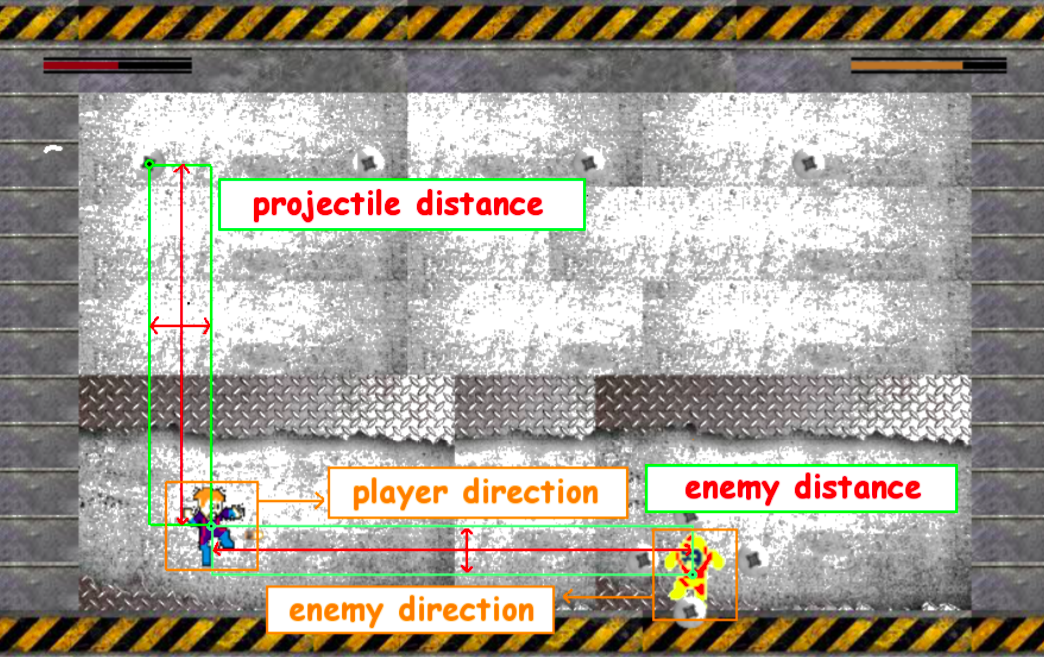
\includegraphics[width=0.5\textwidth]{images/Evoman3.png}
        \caption{Sensors available for the player\cite{evoman}.}
        \label{fig:sensors}
    \end{figure}
    The actions which the agent may take are:
    \begin{itemize}
        \item walk left
        \item walk right
        \item jump
        \item shoot
        \item release of the jump
    \end{itemize}

    The lives of the player and the enemy start at 100.
    Everytime one of them gets hit, their life deplenishes.
    Whoever's life reaches 0 loses the game.

    In the original Capcom game the player would have to beat $8$ opponents and acquire their weapons
    as they are defeated.
    The additional difficulty of EvoMan comes from the fact that the player has to defeat all
    the opponents using only the starting weapon.
    Each opponent can be fought on a specified difficulty level.
    The difficulty level is an integer greater or equal than $1$ which is translated into a factor for the damage
    taken and damage given by the player, the higher the difficulty level the lower the damage given and the higher the damage taken.
    The framework is freely available\footnote{\url{https://github.com/karinemiras/evoman_framework}}
    and it is currently compatible with Python 3.6 and 3.7.
    There is also an extensive documentation
    available\footnote{\url{https://github.com/karinemiras/evoman_framework/blob/master/evoman1.0-doc.pdf}}.

    \subsection{Problem}\label{subsec:problem}
    Beating an opponent is relatively easy when using specialized models against a specific enemy.
    The authors of the EvoMan framework trained multiple specialized agents against all opponents.
    After playing a game, the formula for the gain by which an agent is evaluated is:
    \boldmath
    \begin{gather*}
        gain = 100.01 + player\_life - enemy\_life
    \end{gather*}
    \unboldmath
    The highest final gain is 185.67\cite{evoman} and it was obtained with the NEAT\cite{neat} algorithm. \\

    The problem we are trying to solve is a generalization of the one above.
    We are to train an agent against four enemies and then test its performance against all eight.
    The final score metric of an agent is the harmonic mean of the gains against all enemies.
    The combination of four enemies we are to train the agent is not fixed.
    The difficulty level for solving this problem is $2$ for all enemies in training and testing,
    but we did some exploratory work with greater level of difficulties outside training and
    testing for obtaining the final solution for the problem.

    The specifications above, like the number of enemies chosen for training or the difficulty level,
    come directly from a competition organized by the creators of the framework\cite{evoman_competition}.


    \section{Approach}\label{sec:approach}
    Our intention was to develop a cascade ensemble method where the resulting model of an algorithm
    which can achieve a decent gain fast or has a high exploratory bias is the starting point of an algorithm with high exploitative bias.
    The algorithm we expected to obtain a decent gain fast is a classic Q-learning\cite{q_learning} algorithm. The exploratory algorithms we have considered are genetic algorithms\cite{genetic_algorithm} and particle swarm optimization\cite{pso}.
    The exploitative algorithm we used was Proximal Policy Optimization\cite{ppo}.

    To find the best bootstraping algorithm we have made the following changes, which had no impact in the training and testing for the final solution to the problem:
    \begin{itemize}
        \item we have increased the difficulty from the default 2 to 5.
        \item the evaluation is made only on the second opponent due to the varied environment.
        \item the gain function was modified as in Karine Miras' analysis\cite{evoman_blog} to:
        \boldmath
        \begin{gather*}
            0.9 \cdot (100 - enemy\_life) + 0.1 \cdot player\_life\\
            -\hspace{0.2cm} ln(nr\_of\_game\_timesteps)\\
        \end{gather*}
        \unboldmath
    \end{itemize}

    The best exploratory algorithm would be trained on four enemies and
    used in cascade with proximal policy optimization without the changes mentioned in this section.

    \subsection{Q-Learning}\label{subsec:q-learning}
    The algorithm we expected to obtain a decent gain fast is a classic Q-learning\cite{q_learning} algorithm with neural networks.

    We used a neural network to predict the reward function for each possible move
    (left, right, shoot, jump, release of jump) from a given state.
    We then take the action with the highest predicted reward.
    The input of this neural network is composed of the current game sensors and the
    previous 2 game sensors with the moves taken at that specific point.

    The neural network used for experiments has 2 hidden layers with 32 neurons each.
    Each layer has l2 regularization applied with a weight decay of 0.01 and sigmoid activation.
    After each predicted move, we updated the neural network using backpropagation,
    using as input the game sensors and as output the true reward function.
    A game ends when either the agent or the enemy lose all life.
    We have trained the agent on 5000 games.
    The average number of frames per game for the best model is 287.

    \subsection{Evolving Neural Network Weights with Genetic Algorithms}\label{subsec:evolving-neural-network-weights-with-genetic-algorithms}
    We used genetic algorithms to evolve the weights of neural networks with fixed structures.

    \subsubsection{Sparse Reward Genetic Algorithm}
    The second algorithm is a sparse reward neuroevolution\cite{neuro}.
    The reward is defined as "sparse" because an agent doesn't find out how well it's doing until
    the end of the game, with no feedback during the game.
    An individual is represented as the weights of a neural network.

    The neural network role is to predict the next move using the current game sensors and
    the previous 2 game sensors with the moves taken at that specific point.
    We used 2 hidden layers with 32 neurons for each individual.

    We start with randomly initialized neural network weights and then represent them as a bitstring.
    The weights used for the neural network were values between 2 and -2 with a precision of 6 digits.

    For evaluation, the bitstring is transformed into the weights of the neural network and a game is played,
    from which we can obtain the individual fitness.

    Since we are representing the individuals as bitstrings we were able to apply
    a simple genetic algorithm\cite{genetic_algorithm}.

    The configurations we have used for the genetic algorithm is:
    \begin{itemize}
        \item population size: 50
        \item number of generation: 500
        \item crossover rate: 0.7
        \item mutation rate: \{0.008, 0.1\}
        \item elitism: 1
    \end{itemize}
    We have tried two experiments with different mutation rates in order to observe whether a very high
    mutation rate can lead to good results for the problem. \\

    The solution of the genetic algorithm is the best individual from the last generation.
    Since we have used an elitism of 1, this means that the solution of the genetic algorithm is
    the best individual ever evaluated.

    \subsubsection{Iterative Genetic Algorithm}
    The next algorithm is an iterative neuroevolution.
    It is "iterative" because the agents are trained on a small number of game steps
    first and then the number of game steps slowly increases.

    After a number of generations we increase the number of game timesteps the agents are allowed to train on.
    The fitness function was scaled based on the number of game timesteps in a way that if an agent
    training on x game timesteps will always have a fitness lower than an agent training on y game
    timesteps if x is lower than y.

    \subsection{Searching Neural Network Weights with Particle Swarm Optimization}\label{subsec:searching-neural-network-weights-with-particle-swarm-optimization}
    We have used particle swarm optimization\cite{pso} to search for the weights of a neural network of a
    fixed structure which maximize the fitness defined in this section.
    We used the same neural network configuration as in the case of genetic algorithms. \\

    The configurations used for the particle swarm optimization\cite{pso} algorithm are:
    \begin{itemize}
        \item population size: 30
        \item number of iterations: 200
        \item cognitive weight: \{0.4, 0.8, 1.5\}
        \item social weight: \{0.8, 0.4, 3\}
        \item inertia weight: \{constant 1, decreasing from 1 by 0.0035 every epoch\}
    \end{itemize}

    The same separation between an sparse and an iterative search was made in the case
    of particle swarm optimization, as in the case of the genetic algorithms.

    We also tried to search with pso using an uniformly decreasing inertia weight with respect
    to the percent of the iterations passed, having values from 1 to 0.3. The inertia weight controls the level of exploration versus exploitation, higher values in the beginning of the algorithm lead to better exploration while lower values towards the end of the algorithm lead to better exploitation.
    This was tried to make the PSO focus even more on exploitation, rather than exploration.

    \subsection{Proximal Policy Optimization}\label{subsec:proximal-policy-optimization}
    PPO\cite{ppo} is the algorithm we have used for exploitation.
    For this stage we have used the default difficulty of 2, the training was done on 4 opponents
    and the evaluation was done as described in the Problem Description(\ref{sec:problem-description}).

    The neural network is randomly initialized. \\
    The configuration we have used for the PPO is:
    \begin{itemize}
        \item hidden layers: (64, 64)
        \item steps per epoch: 10000
        \item epochs: 3000
        \item gamma: 0.99
        \item clip\_ratio: 0.2
        \item pi\_lr: 3e-4
        \item vf\_lr: 1e-3
        \item train\_pi\_iterations: 80
        \item train\_v\_iterations: 80
        \item lambda: 0.97
        \item target\_KL: 0.01
    \end{itemize}

    \subsection{Particle Swarm Optimization Cascaded With Proximal Policy Optimization}\label{subsec:particle-swarm-optimization-cascaded-with-proximal-policy-optimization}
    The output weights of a neural network resulted from a PSO search is the starting agent for PPO\@.
    In order to solve the generalized problem we have made the following changes from the PSO from the exploratory stage:
    \begin{itemize}
        \item The sizes of the hidden layers were increased from (32, 32) to (64, 64).
        \item It is trained on four opponents, not only one.
        \item The fitness function is the one from the Problem Description (\ref{sec:problem-description}).
    \end{itemize}
    The same configuration was used for PPO as in the case of the PPO with random
    weights initialization.


    \section{Experimental Investigation}\label{sec:experimental-investigation}

    \subsection{Q-Learning}\label{subsec:q-learning2}
    The Q-learning algorithm was the starting point of our comparison.
    Even when trained and evaluated against the same opponent, it would lose every game
    while inflicting almost no damage.

    \subsection{Genetic Algorithms}\label{subsec:genetic-algorithms}
    The iterative genetic algorithm leads to much better results than Q-learning (Fig.~\ref{fig:q_vs_ga_iterative}).
    \begin{figure}[!h]
        \centering
        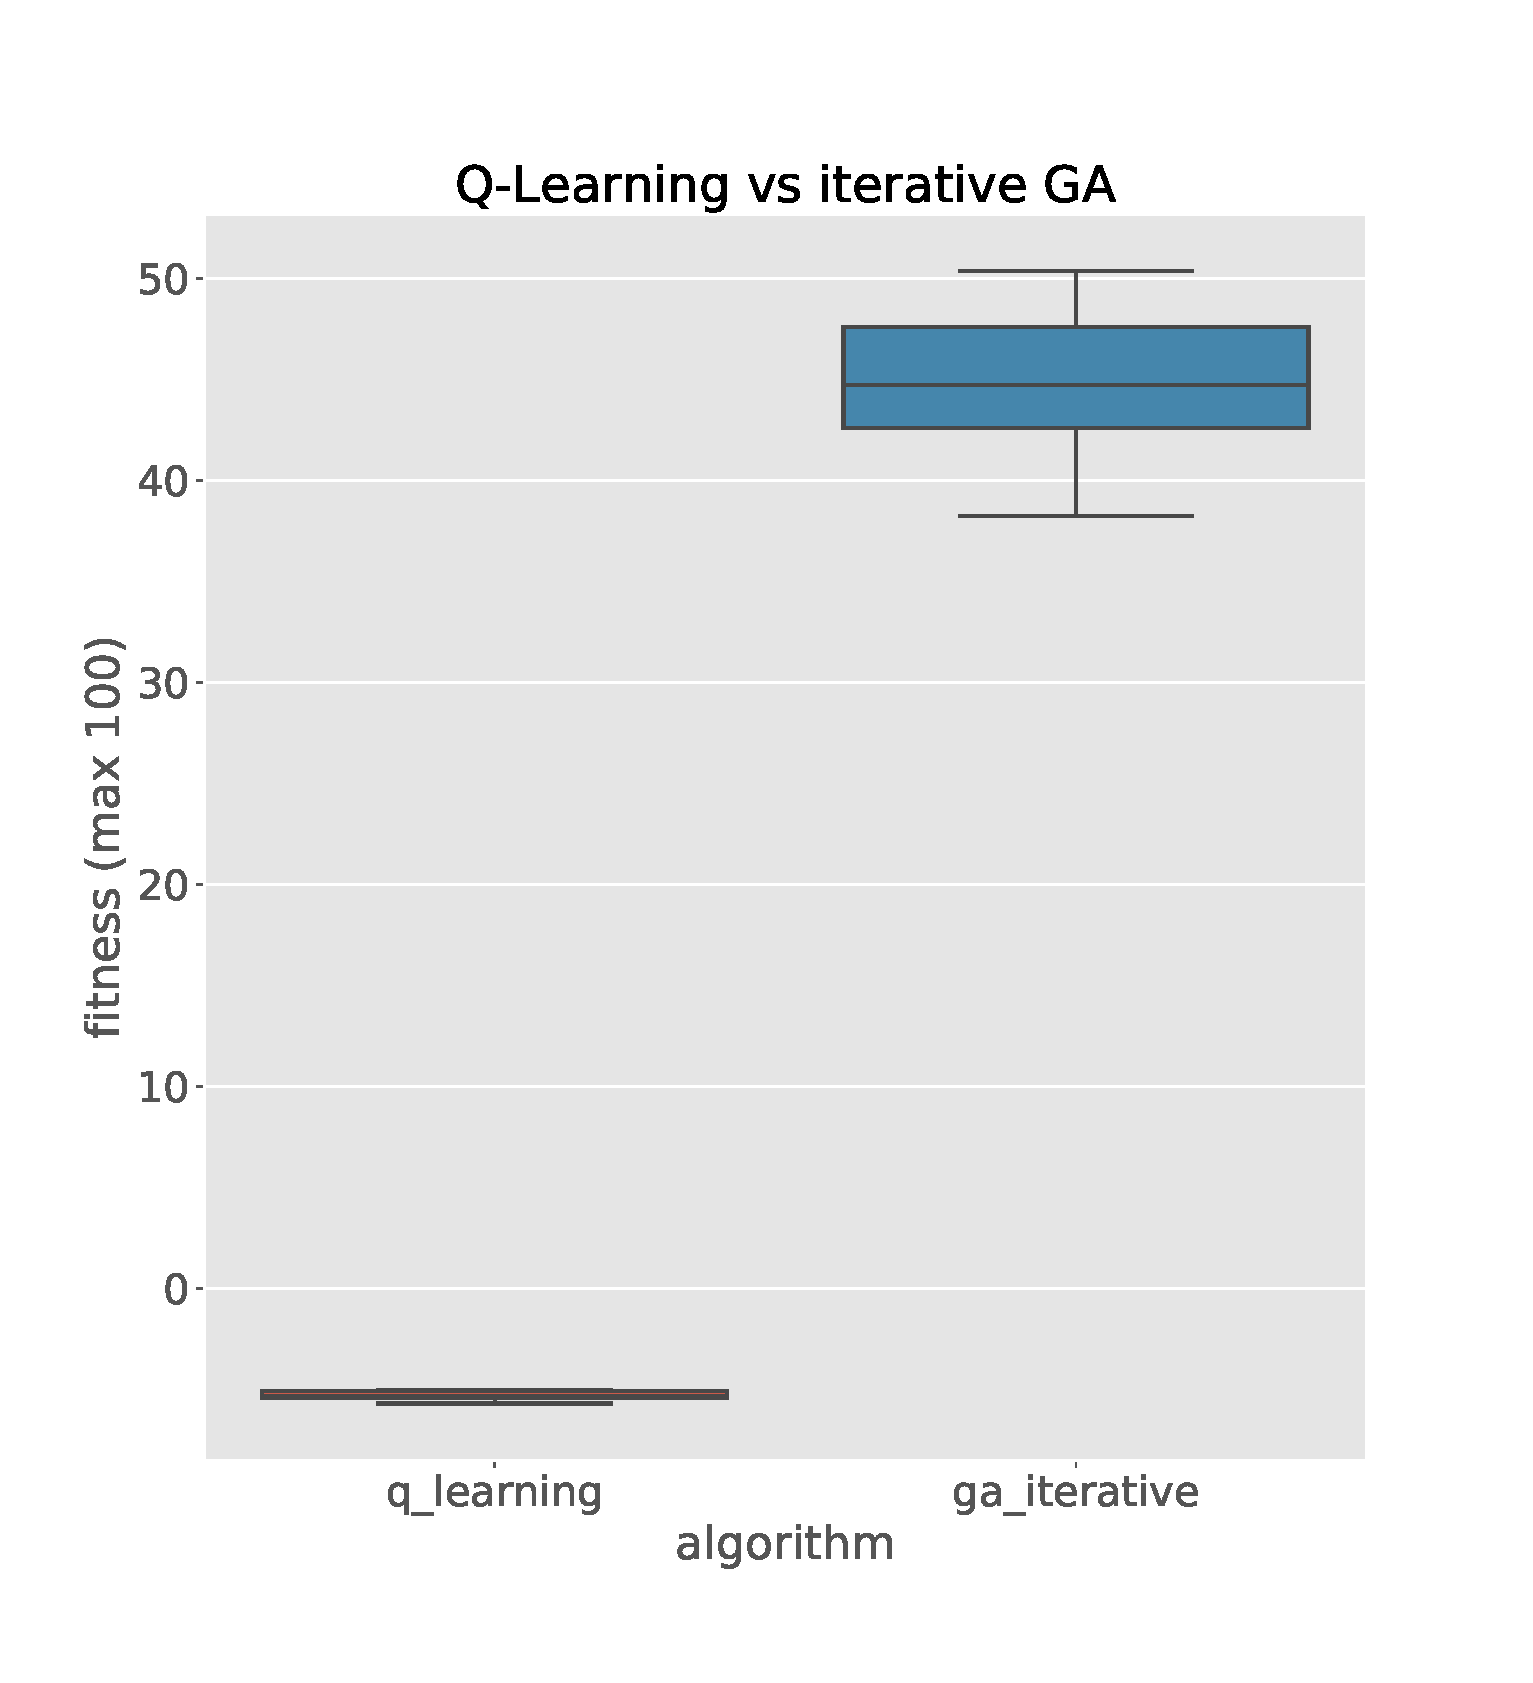
\includegraphics[width=0.5\textwidth]{old_images/q_vs_ga_iterative.eps}
        \caption{The fitness comparison between Q-learning and iterative genetic algorithms.}
        \label{fig:q_vs_ga_iterative}
    \end{figure}

    We have shown that a mutation rate of 0.008 leads to better results than a mutation rate of 0.1 (Fig.~\ref{fig:ga_mutation_rates}).
    \begin{figure}[!h]
        \centering
        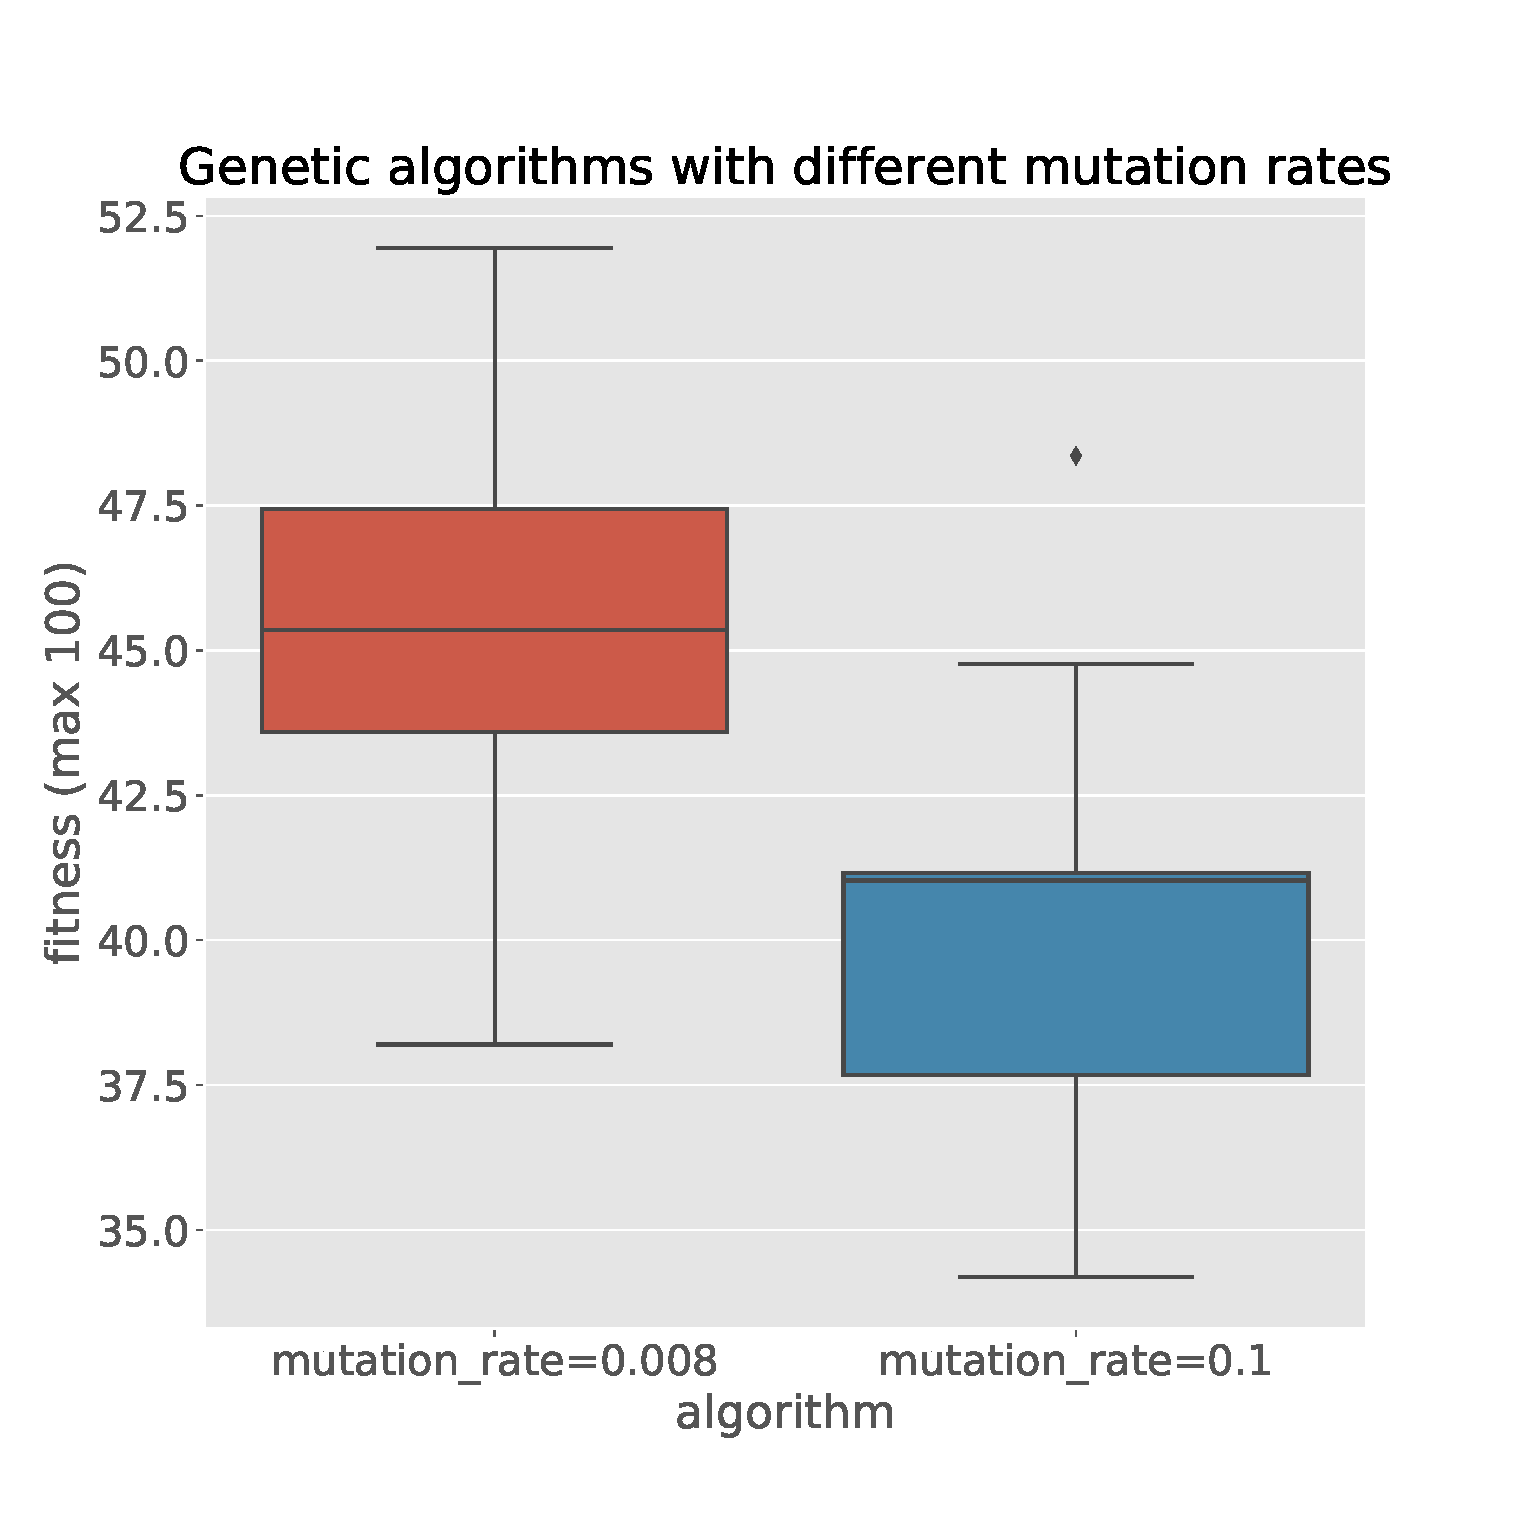
\includegraphics[width=0.5\textwidth]{old_images/ga_mutation_rates.eps}
        \caption{The fitness comparison between sparse genetic algorithms with mutation rate of 0.1 and 0.008.}
        \label{fig:ga_mutation_rates}
    \end{figure}

    The results of the sparse genetic algorithm and the iterative genetic algorithm
    are not significantly different (Fig.~\ref{fig:overview}).

    \subsection{Particle Swarm Optimization}\label{subsec:sparse-particle-swarm-optimization}
    Both particle swarm optimization algorithms lead to much better results than either of the
    sparse and iterative genetic algorithms.
    The iterative PSO lead to worse results than the sparse PSO\@.
    In Fig.~\ref{fig:overview} we can see that the best exploratory algorithm is the sparse PSO\@.
    \begin{figure}[!h]
        \centering
        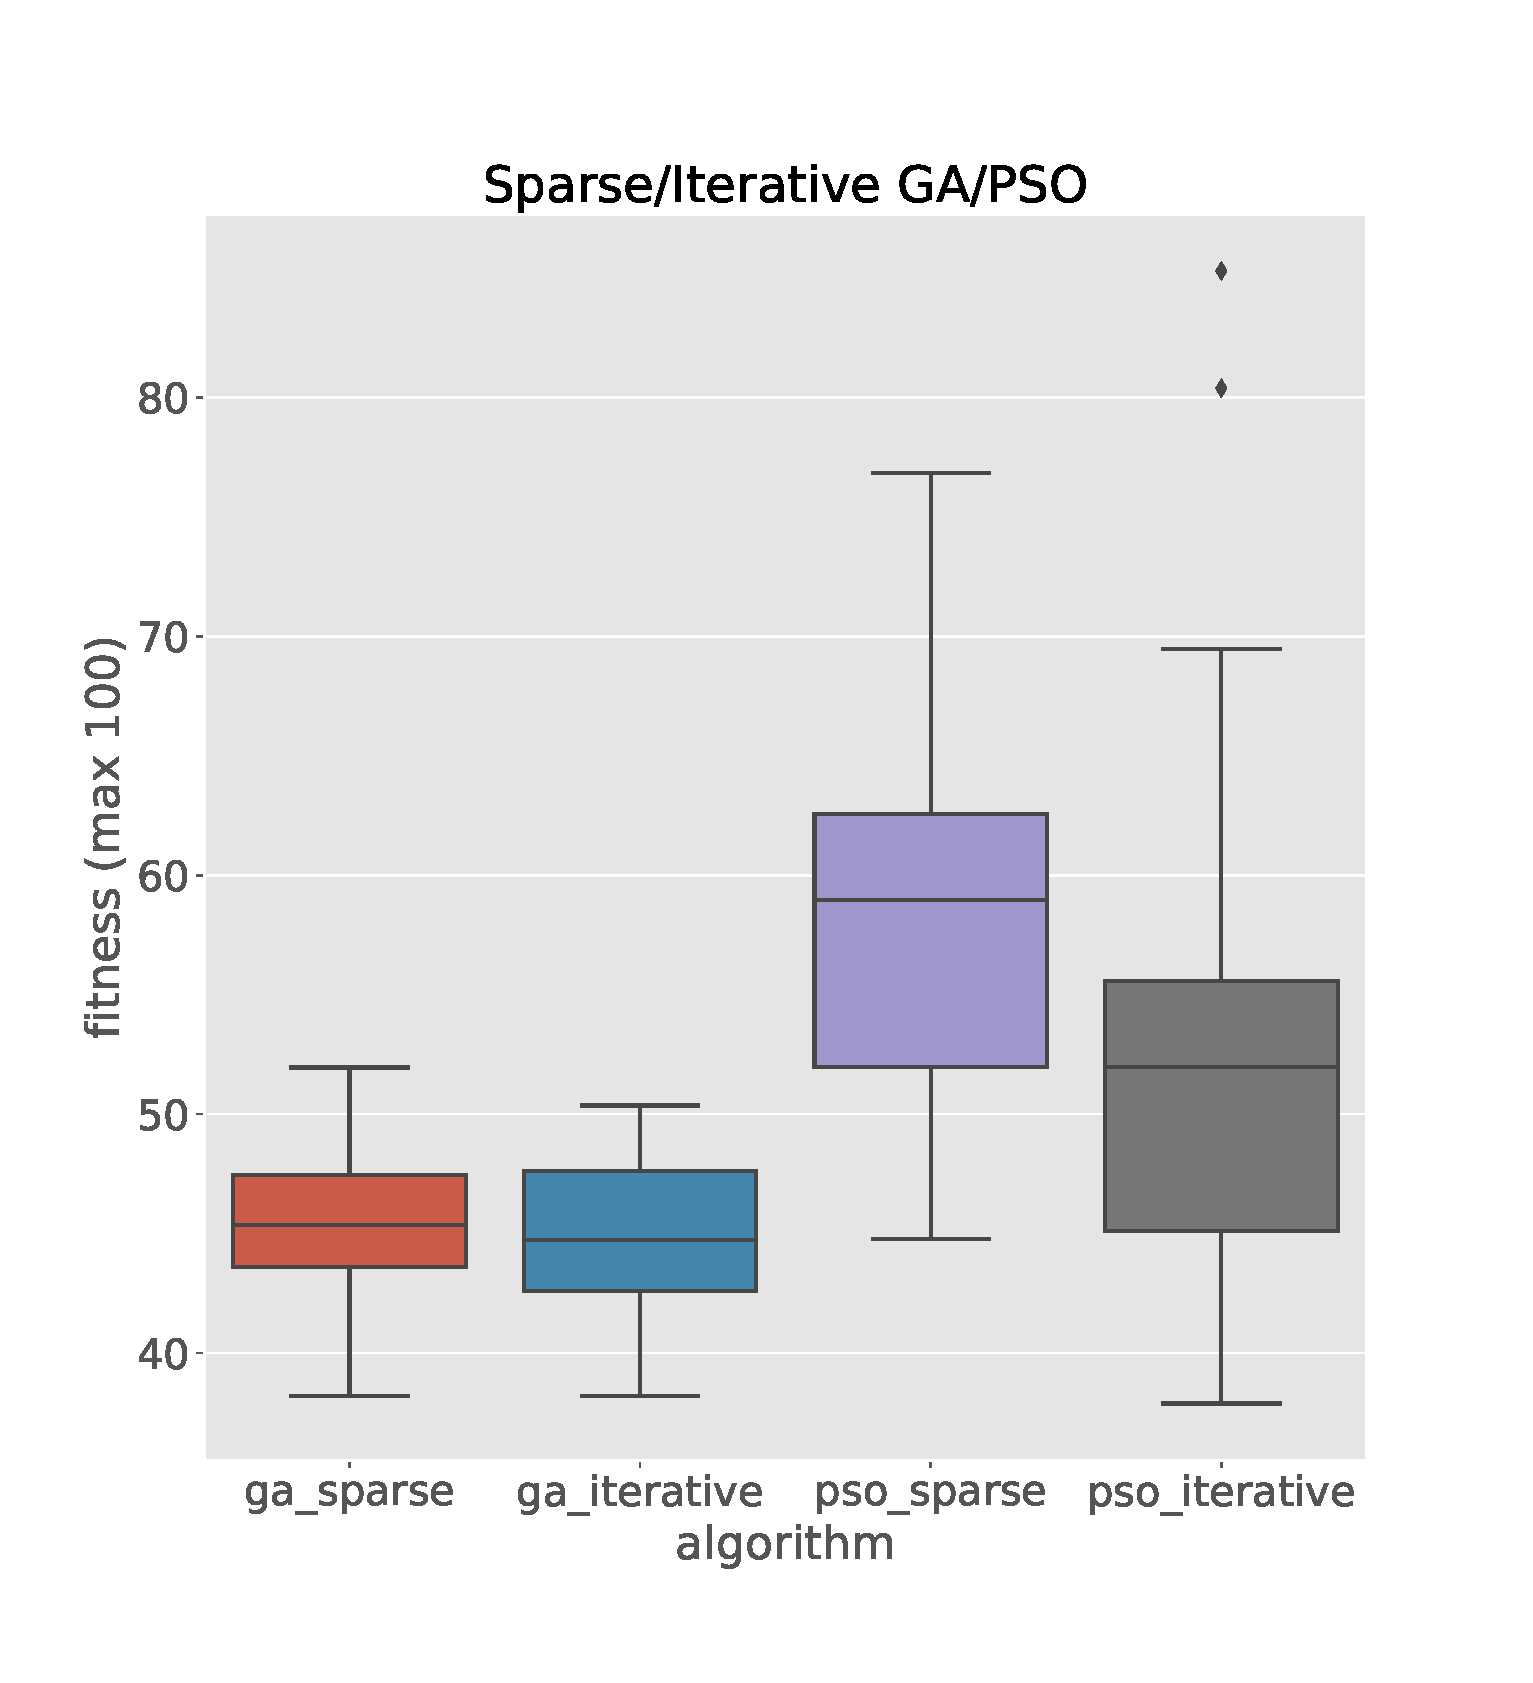
\includegraphics[width=0.5\textwidth]{old_images/overview.eps}
        \caption{The fitness comparison between the iterative and the sparse approached,
        both for the genetic algorithms and the PSO. }
        \label{fig:overview}
    \end{figure}

    The time advantage of iterative PSO vs sparse PSO is not significant (Fig.~\ref{fig:pso_sparse_vs_iterative_time}).
    \begin{figure}[!h]
        \centering
        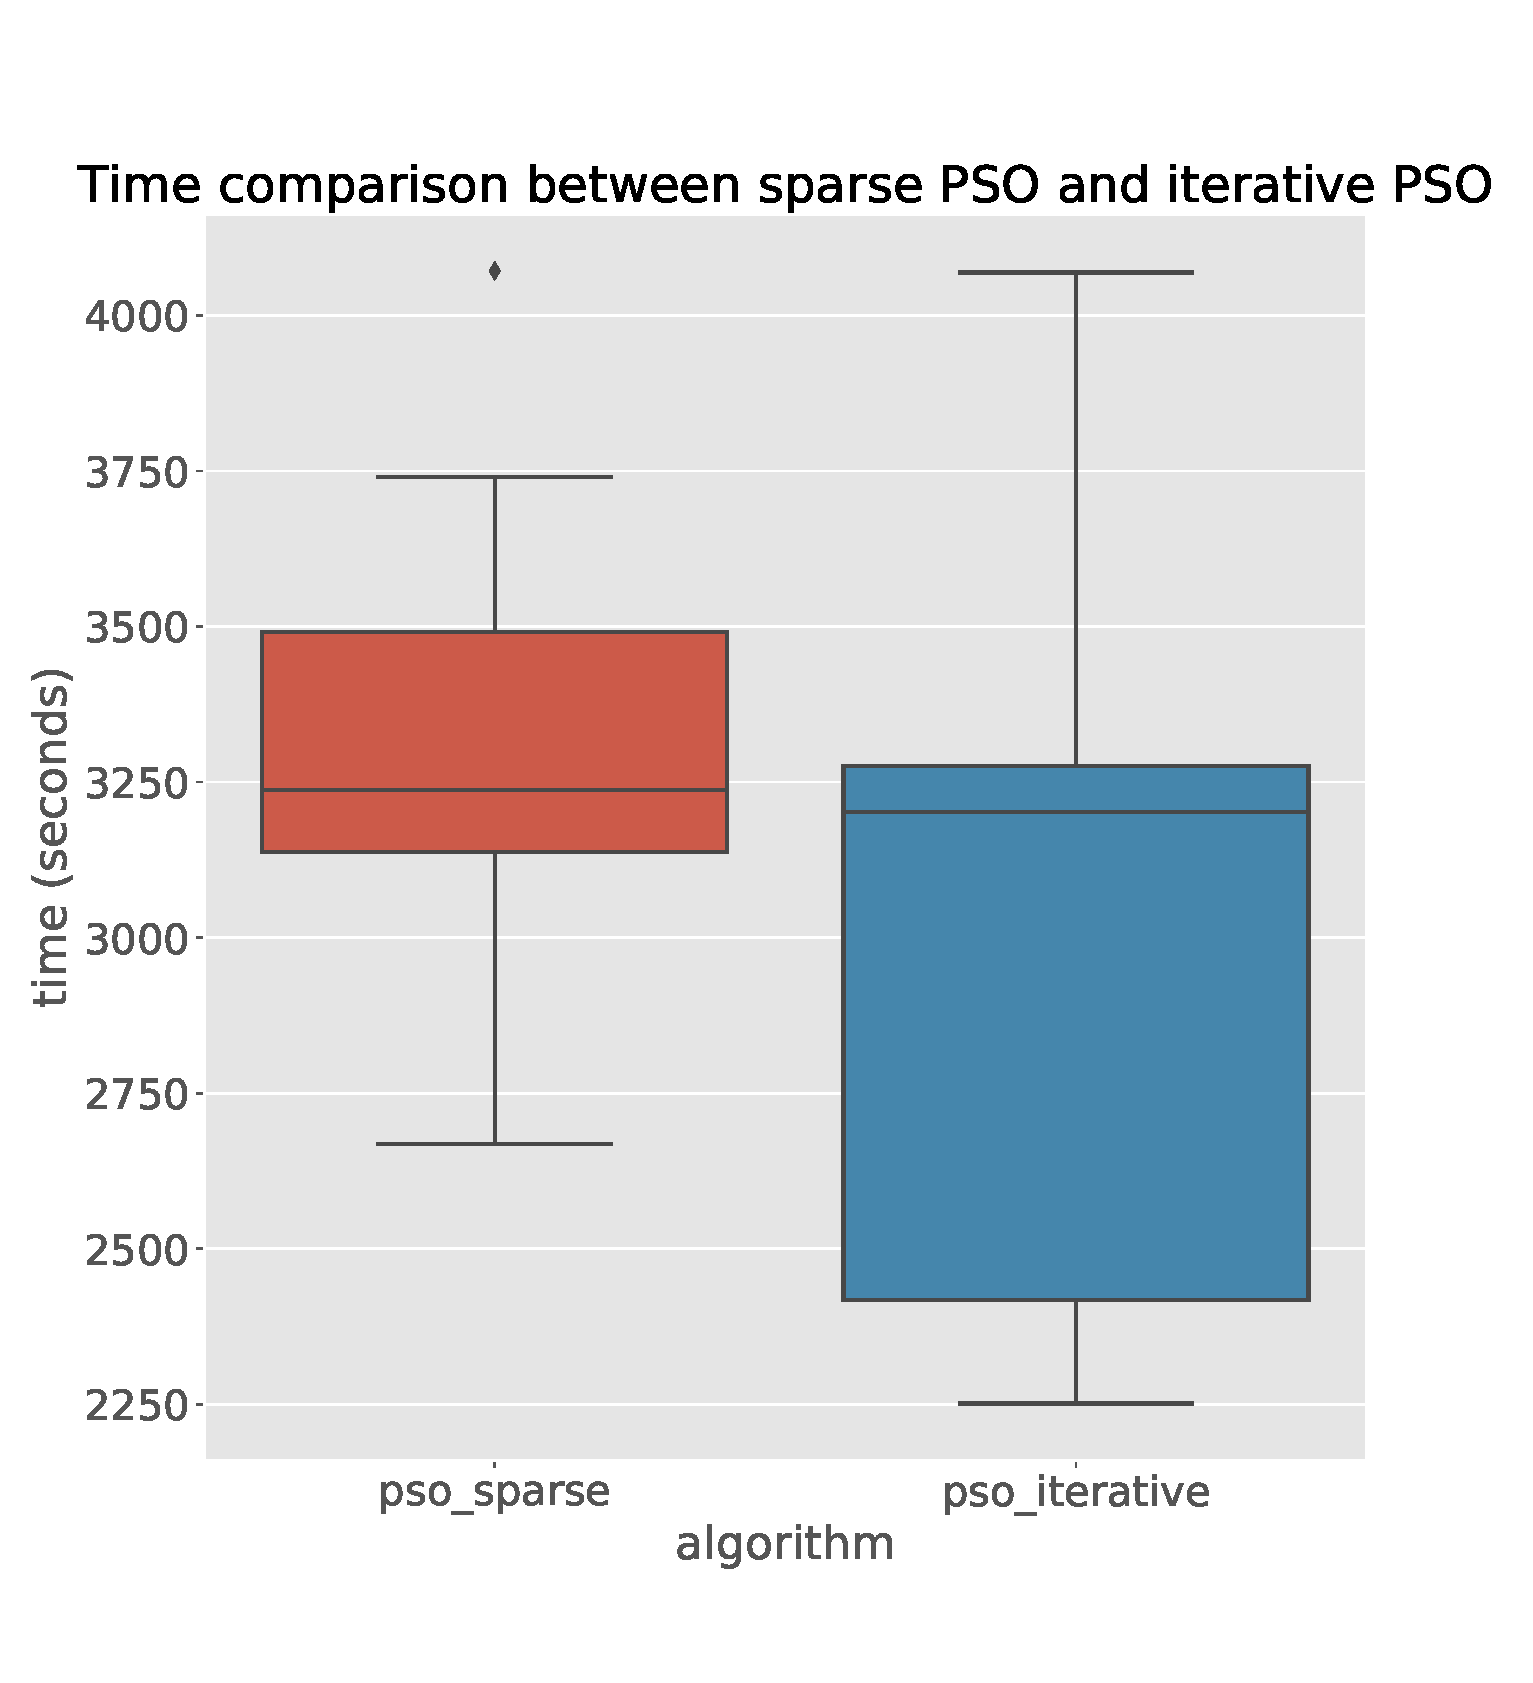
\includegraphics[width=0.5\textwidth]{old_images/pso_sparse_vs_iterative_time.eps}
        \caption{The time comparison between sparse and iterative PSO.}
        \label{fig:pso_sparse_vs_iterative_time}
    \end{figure}

    We have also searched for good PSO weights for our problem.
    In the next stages we have used a cognitive weight of 0.4 and a social weight of 0.8 due to
    its higher variance in results (Fig.~\ref{fig:pso_configs}).

    \begin{figure}[!h]
        \centering
        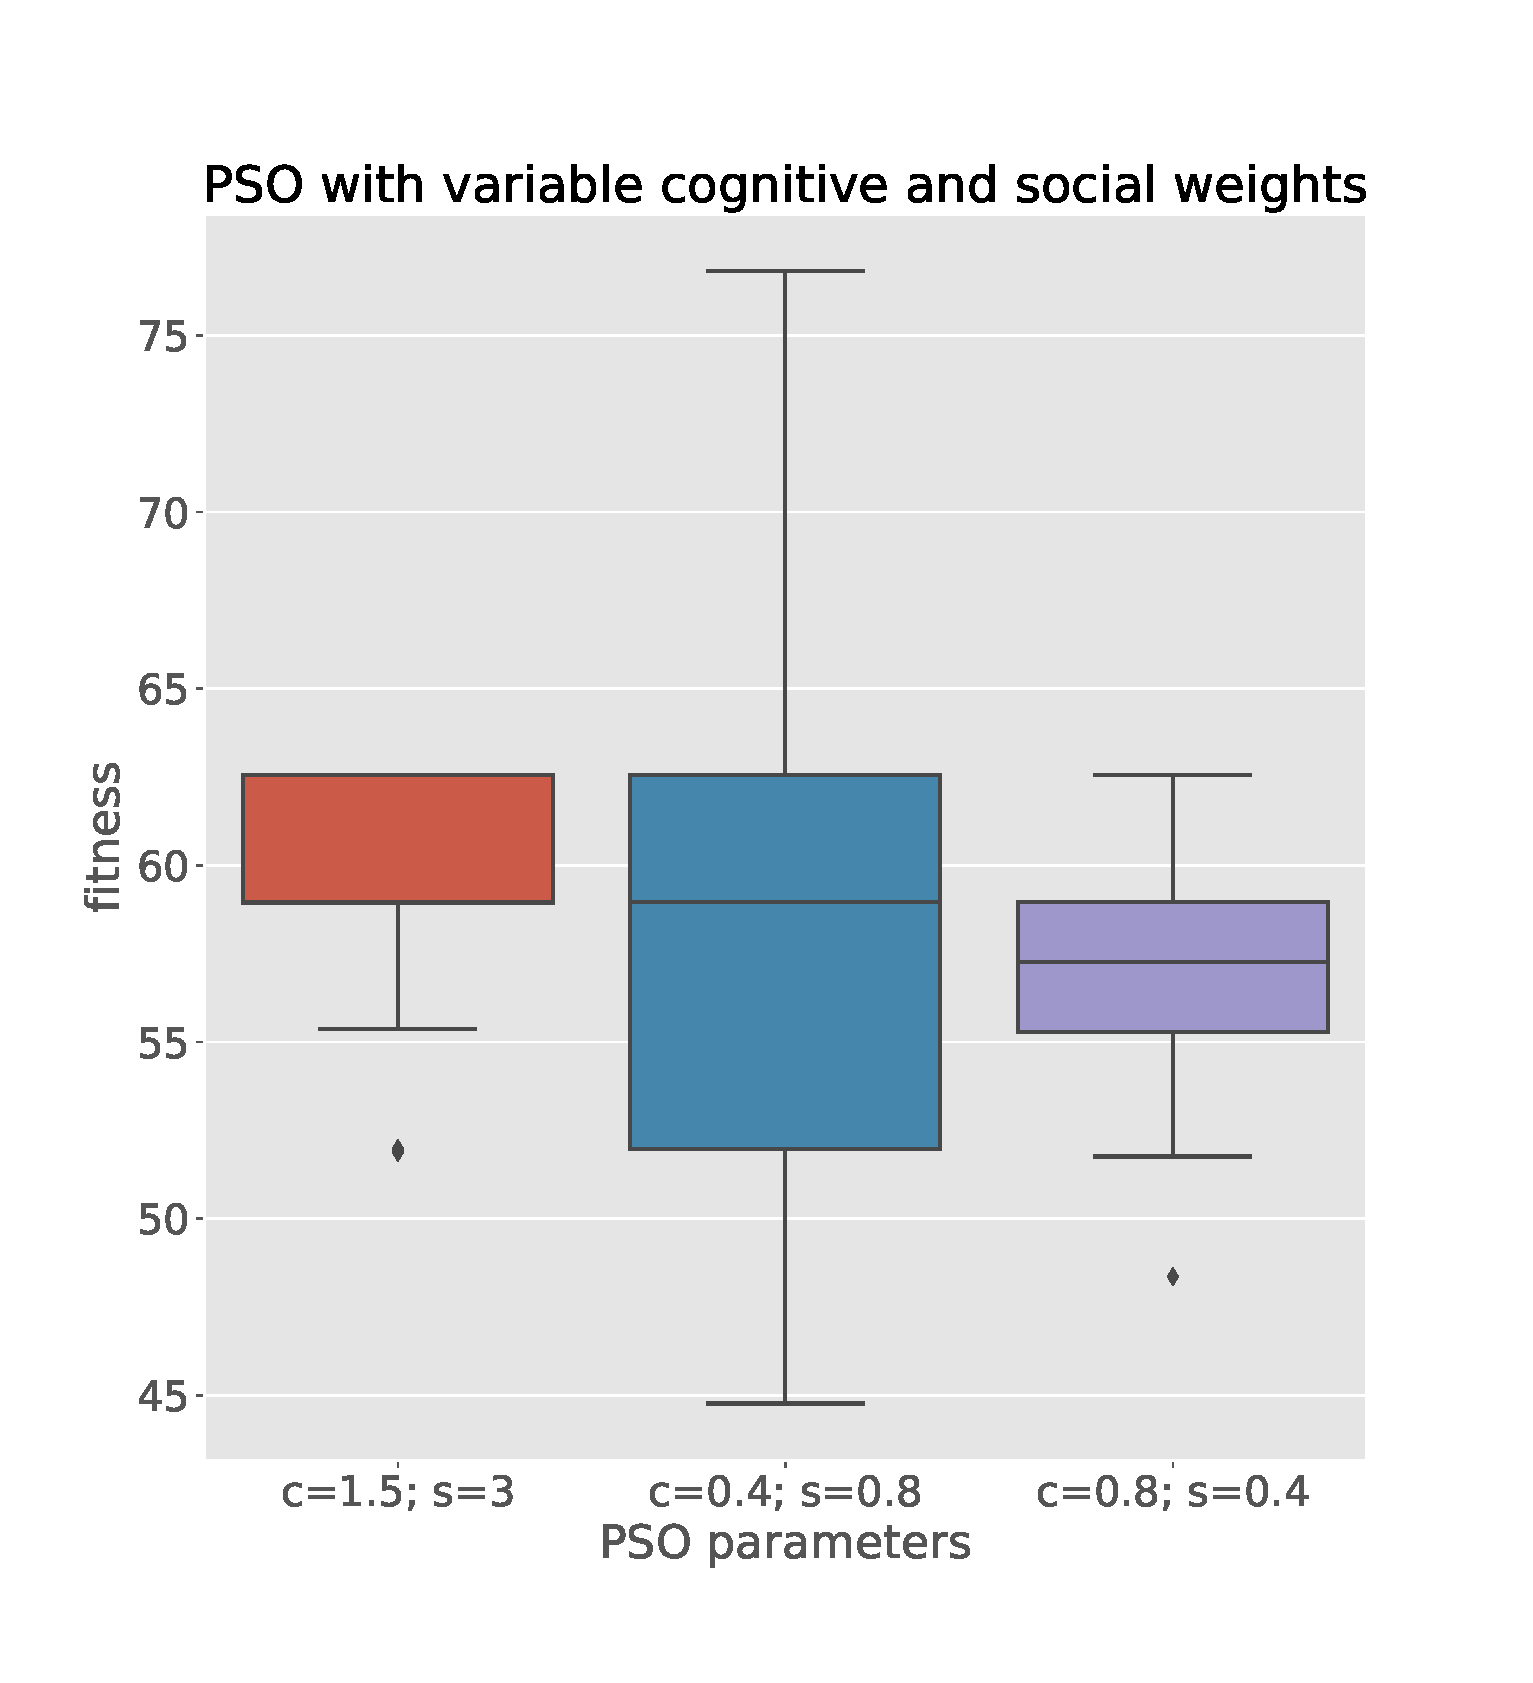
\includegraphics[width=0.5\textwidth]{old_images/pso_configs.eps}
        \caption{The fitness comparison between sparse PSO with different cognitive and social weights.}
        \label{fig:pso_configs}
    \end{figure}

    We have also tried two PSO inertia weight updates (Fig.~\ref{fig:pso_inertia}).
    We continued with the constant inertia weight approach.

    \begin{figure}[!h]
        \centering
        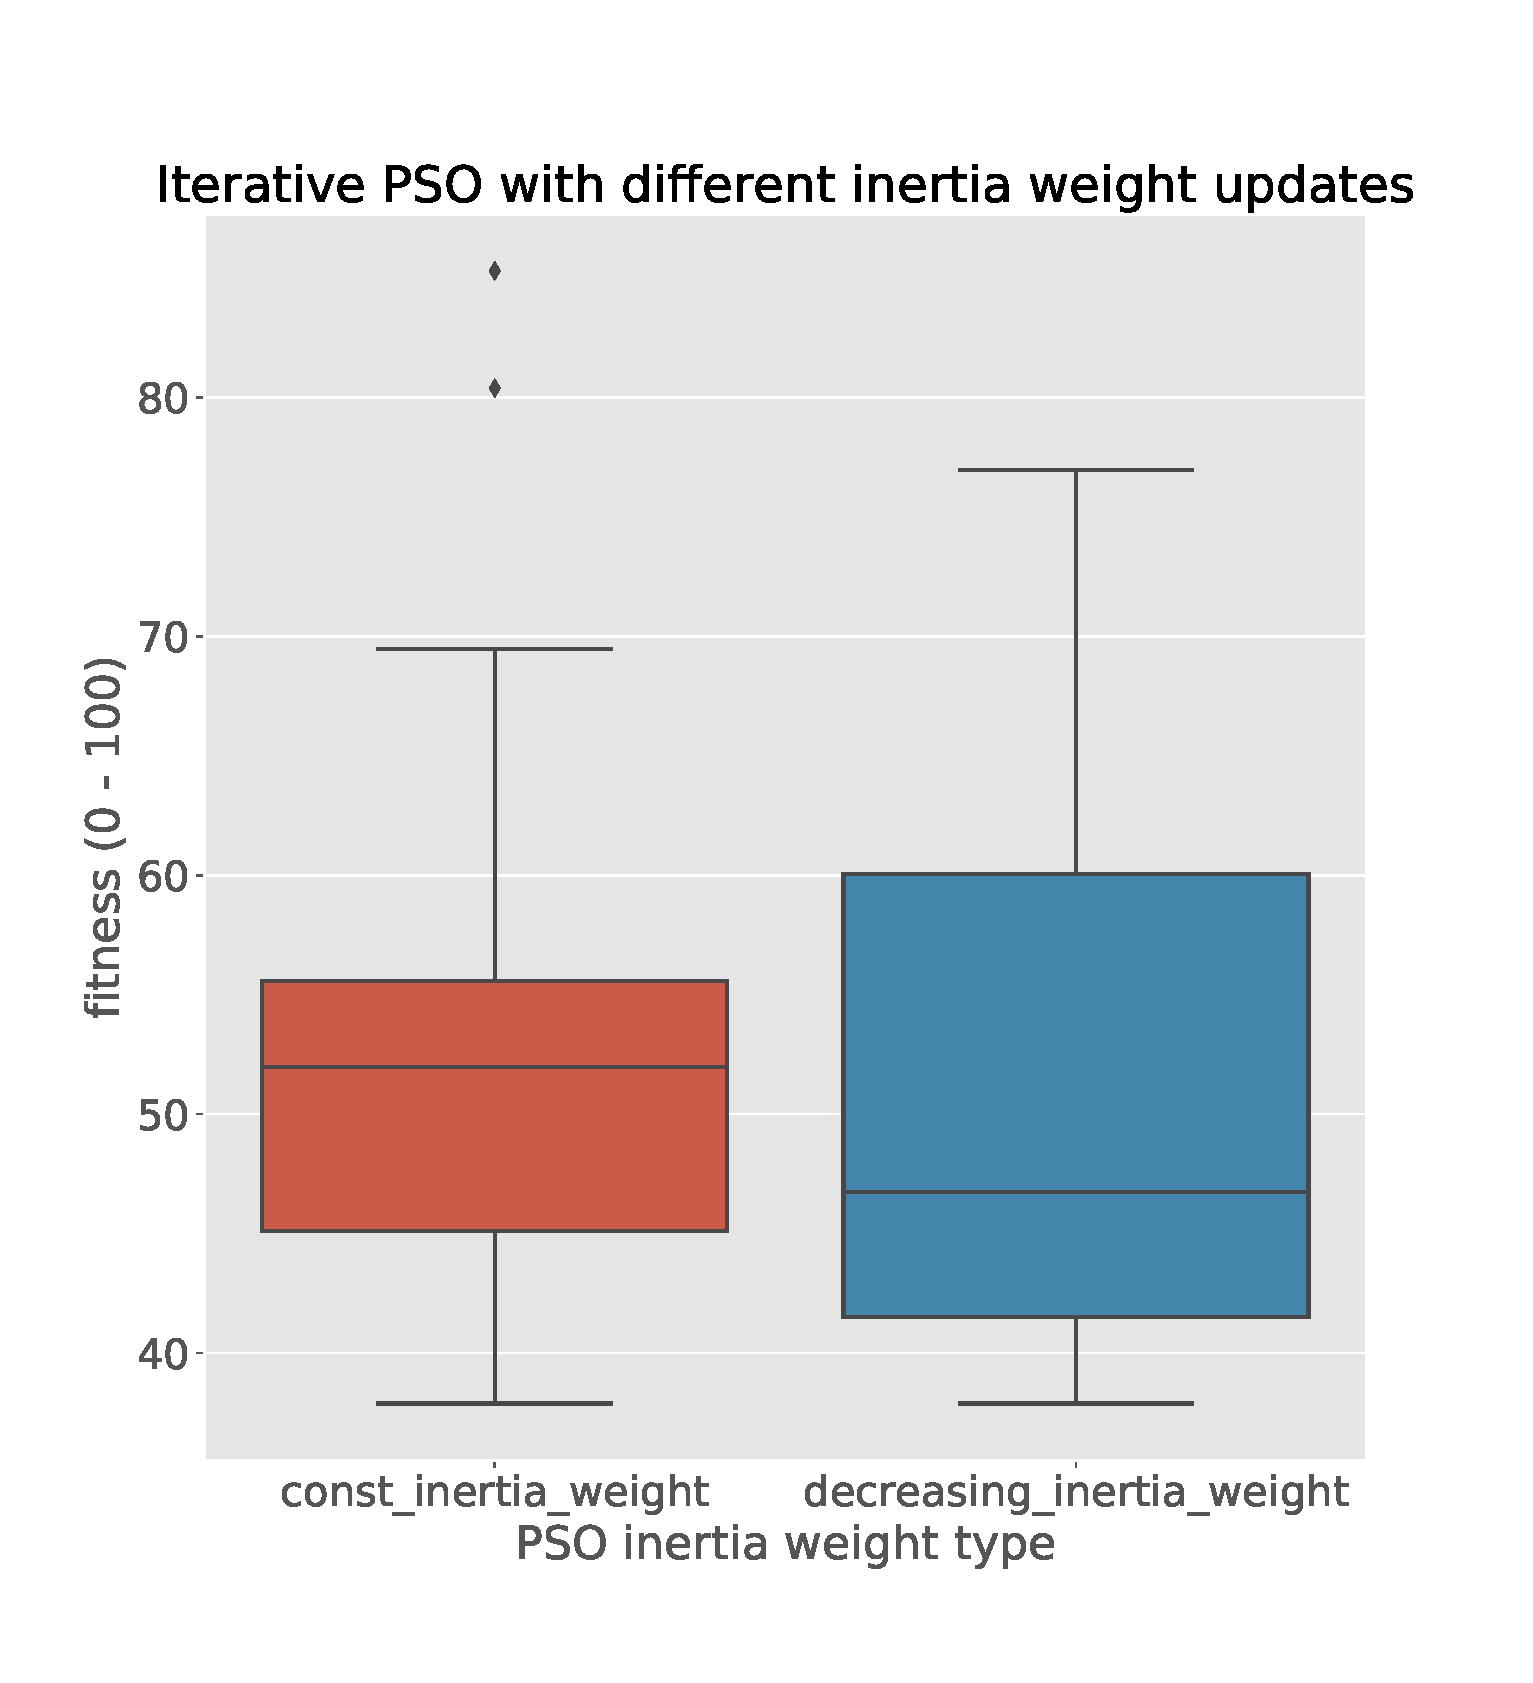
\includegraphics[width=0.5\textwidth]{old_images/pso_inertia.eps}
        \caption{The fitness comparison between PSO with constant inertia
        weight and with uniformly decreasing in time inertia weight.}
        \label{fig:pso_inertia}
    \end{figure}

    After deciding what the starting model should be, we have tested its performance (Fig.~\ref{fig:pso_levels})
    and run time (Fig.~\ref{fig:pso_levels_time}) on multiple difficulties.

    \begin{figure}[!h]
        \centering
        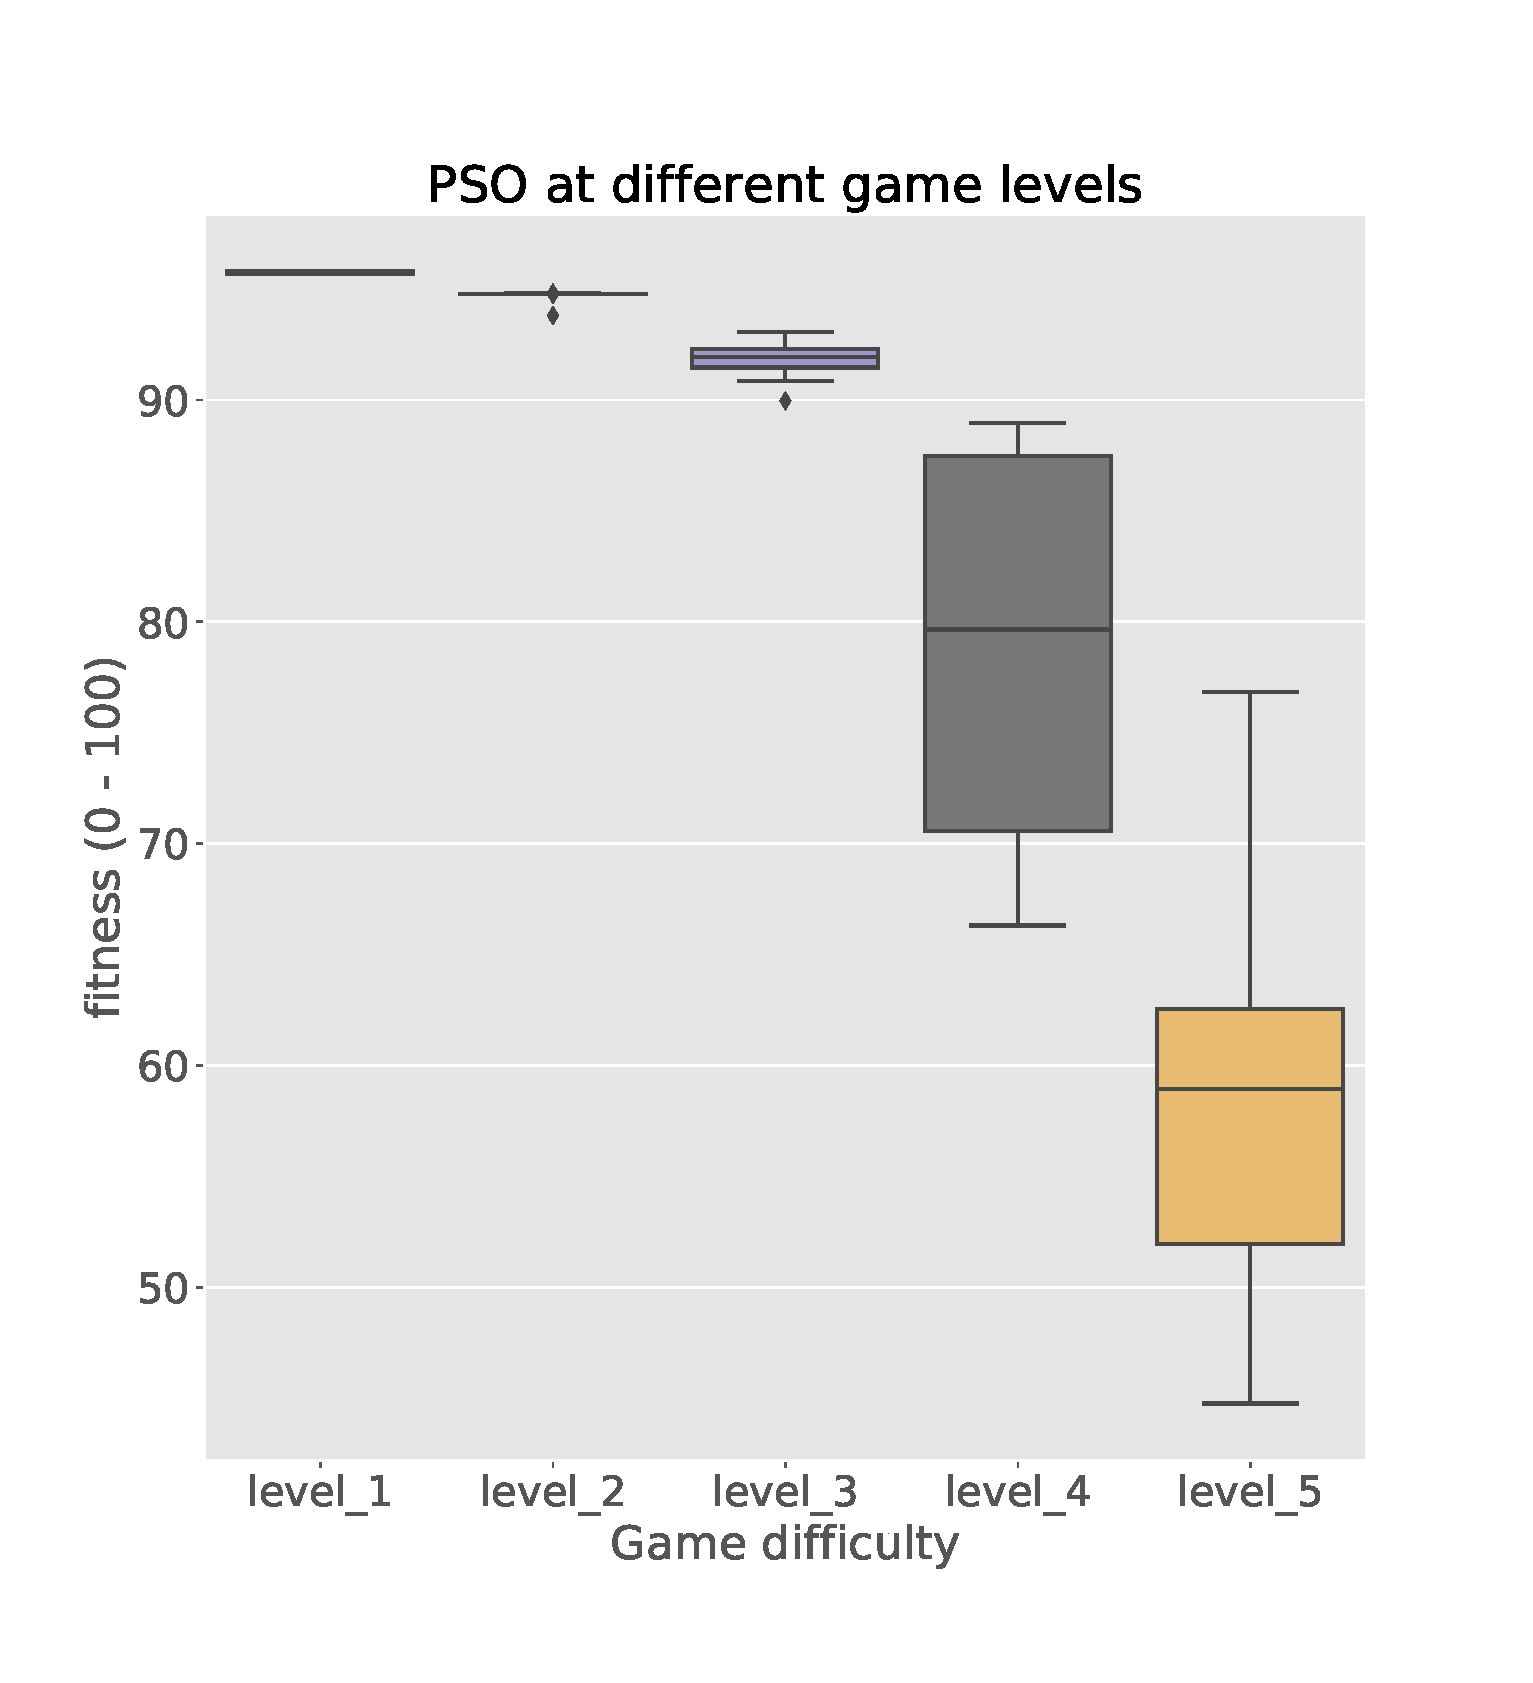
\includegraphics[width=0.5\textwidth]{old_images/pso_levels.eps}
        \caption{The fitness comparison of PSO against different game difficulty levels.}
        \label{fig:pso_levels}
    \end{figure}


    \begin{figure}[!h]
        \centering
        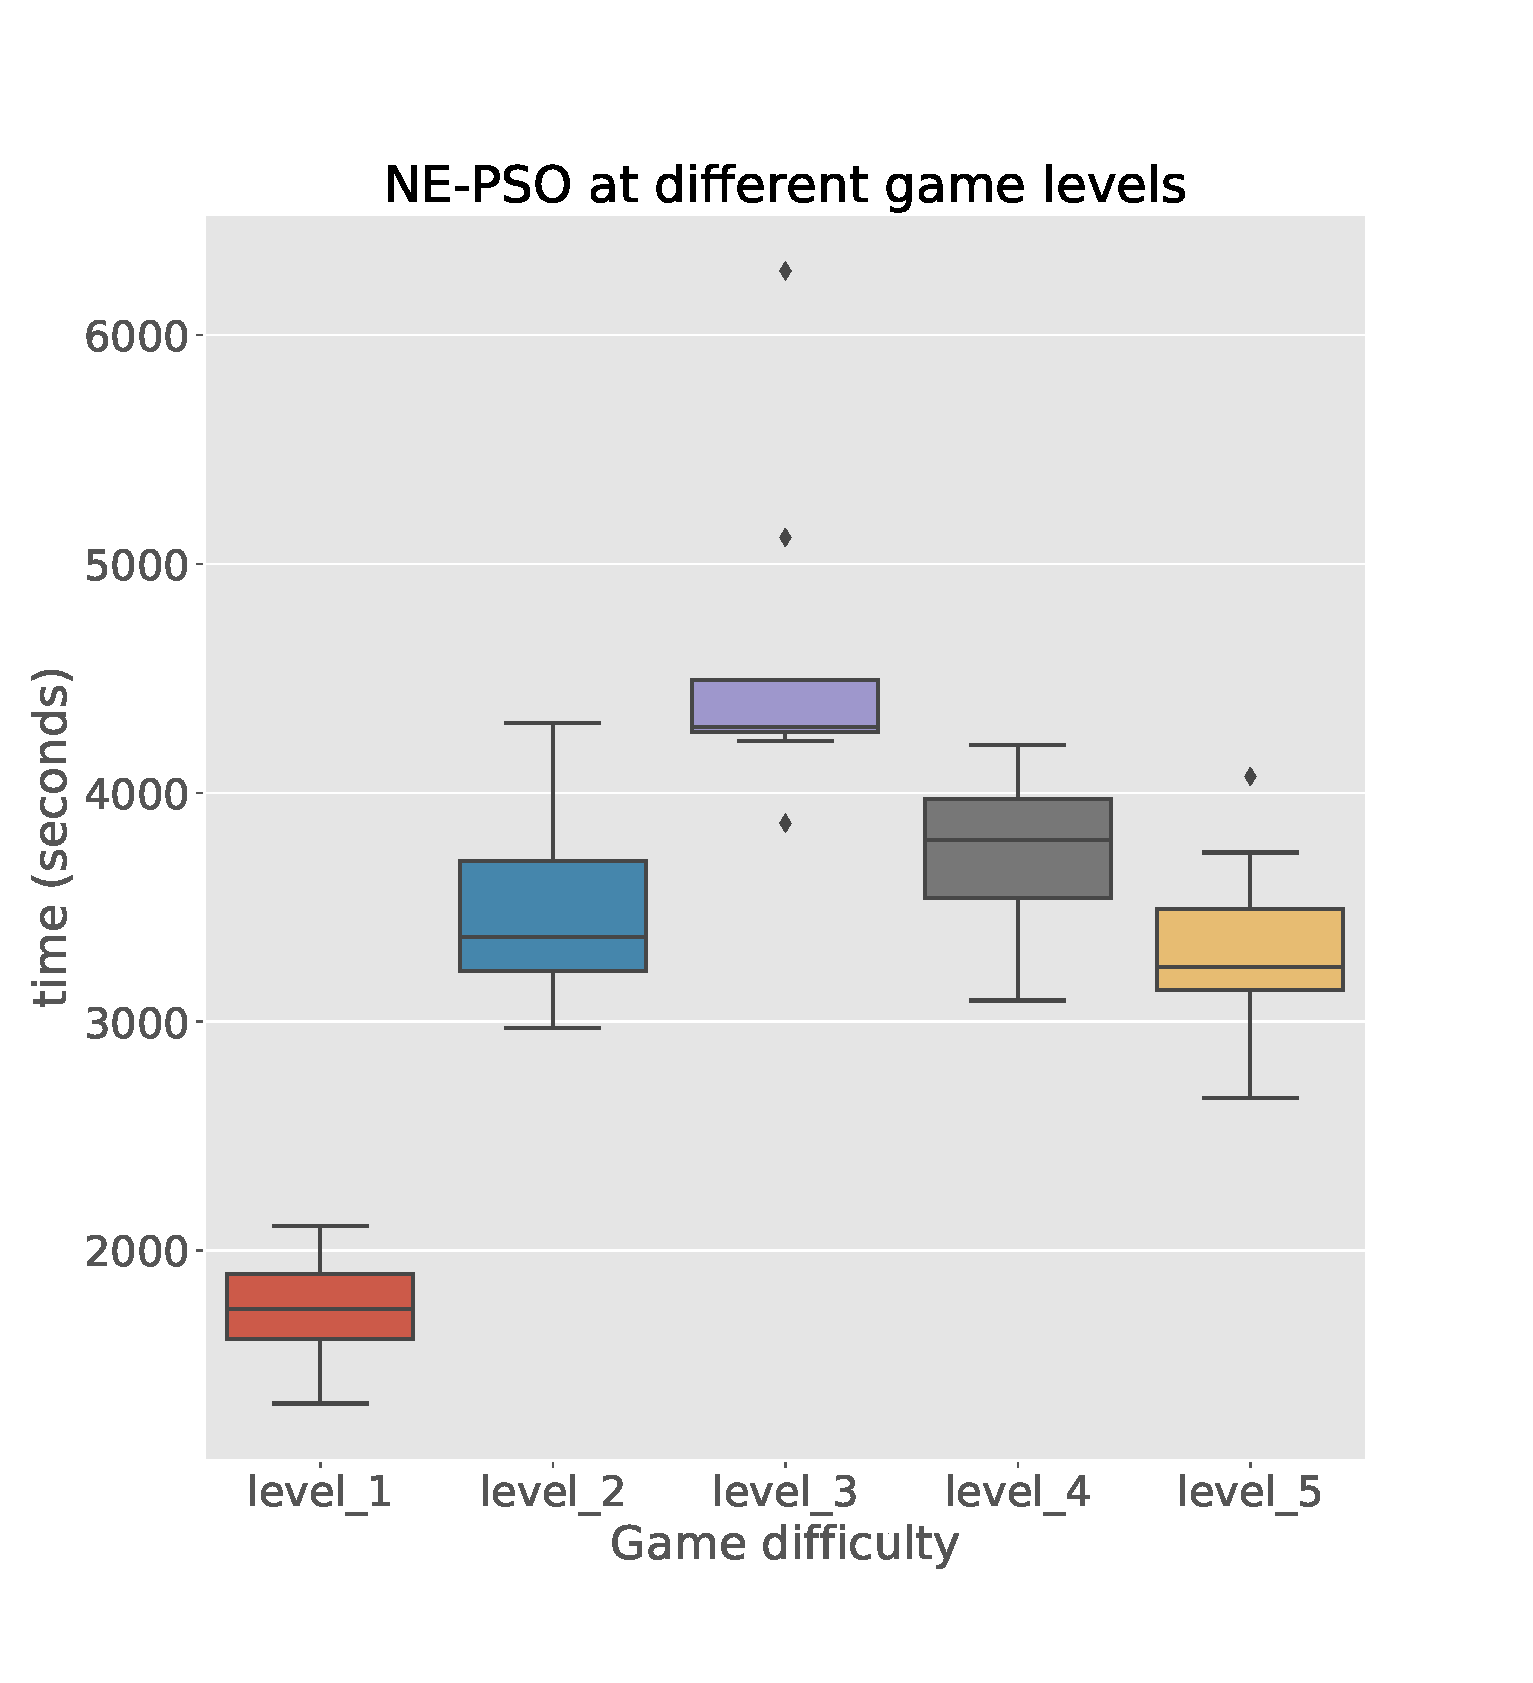
\includegraphics[width=0.5\textwidth]{old_images/pso_levels_time.eps}
        \caption{The time comparison of PSO at different game difficulty levels.}
        \label{fig:pso_levels_time}
    \end{figure}


    \section{Results}\label{sec:results}
    For evaluation of an agent, we ran 30 games against each opponent, leading to 8 averages
    (one per opponent), of which we computed the harmonic mean which is the final result of the agent.

    \subsection{Best Combination of Opponents for Training}\label{subsec:best-combination-of-opponents-for-training}
    We searched for the opponents that lead to the best results.
    The first combination of train opponents we considered was \{1, 2, 6, 7\} which was chosen empirically after manually playing against every opponent and chosing the ones which behaved in such a way that covered the most general concepts our agents could learn in our opinion.
    We observed its final gain as 125.37.
    We realized a set of exploratory experiments where we would search for other combinations of train opponents,
    but starting with the resulting model of PPO trained for 1000 epochs on the combination of opponents \{1, 2, 6, 7\}.
    If by starting with a pre-trained model another combination of train enemies does not lead to better results,
    then we can believe that the respective combination does not lead to better results than \{1, 2, 6, 7\}.
    \begin{table}[htbp]
        \caption{Results for various opponents when starting with a pre-trained PPO model on enemies \{1, 2, 6, 7\}}
        \begin{center}
            \begin{tabular}{|c|c|}
                \hline
                \textbf{Train opponents}&{\textbf{gain (harmonic mean)}} \\
                \hline
                $\{1, 2, 6, 7\} \cup \{3, 4, 5, 8\}$ & $44.16$ \\
                $\{1, 2, 6, 7\} \cup \{3, 4, 6, 7\}$ & $75.3$ \\
                $\{1, 2, 6, 7\} \cup \{1, 3, 6, 7\}$ & $110.19$ \\
                $\{1, 2, 6, 7\} \cup \{2, 3, 6, 7\}$ & $136.1$ \\
                $\{1, 2, 6, 7\} \cup \{2, 4, 6, 7\}$ & $85.22$ \\
                \hline
            \end{tabular}
            \label{table:variations_of_opponents}
        \end{center}
    \end{table}
    \\
    The only combination that lead to a better score than 125.37 was \{2, 3, 6, 7\}.
    We ran an experiment with PPO with random initialization with the combination of train enemies \{2, 3, 6, 7\} and
    we obtained a final gain of 99.97.
    This means that we did not find a better combination of train opponents than \{1, 2, 6, 7\}, so it is the one
    we used for the following experiments.

    \subsection{Random Initialization PPO vs PSO Cascading PPO}\label{subsec:random-initialization-ppo-vs-pso-cascading-ppo}
    The best PSO configuration was used in cascade before the PPO in 4 runs.
    PPO with random initialization was ran 3 times.
    The small number of runs is due to the long run time of the training.
    The worst result of the PPO with random initialization is higher than the best result
    of PSO cascaded with PPO\@ (Fig.~\ref{fig:random_vs_pso_initialization}).
    \begin{figure}[htbp]
        \centering
        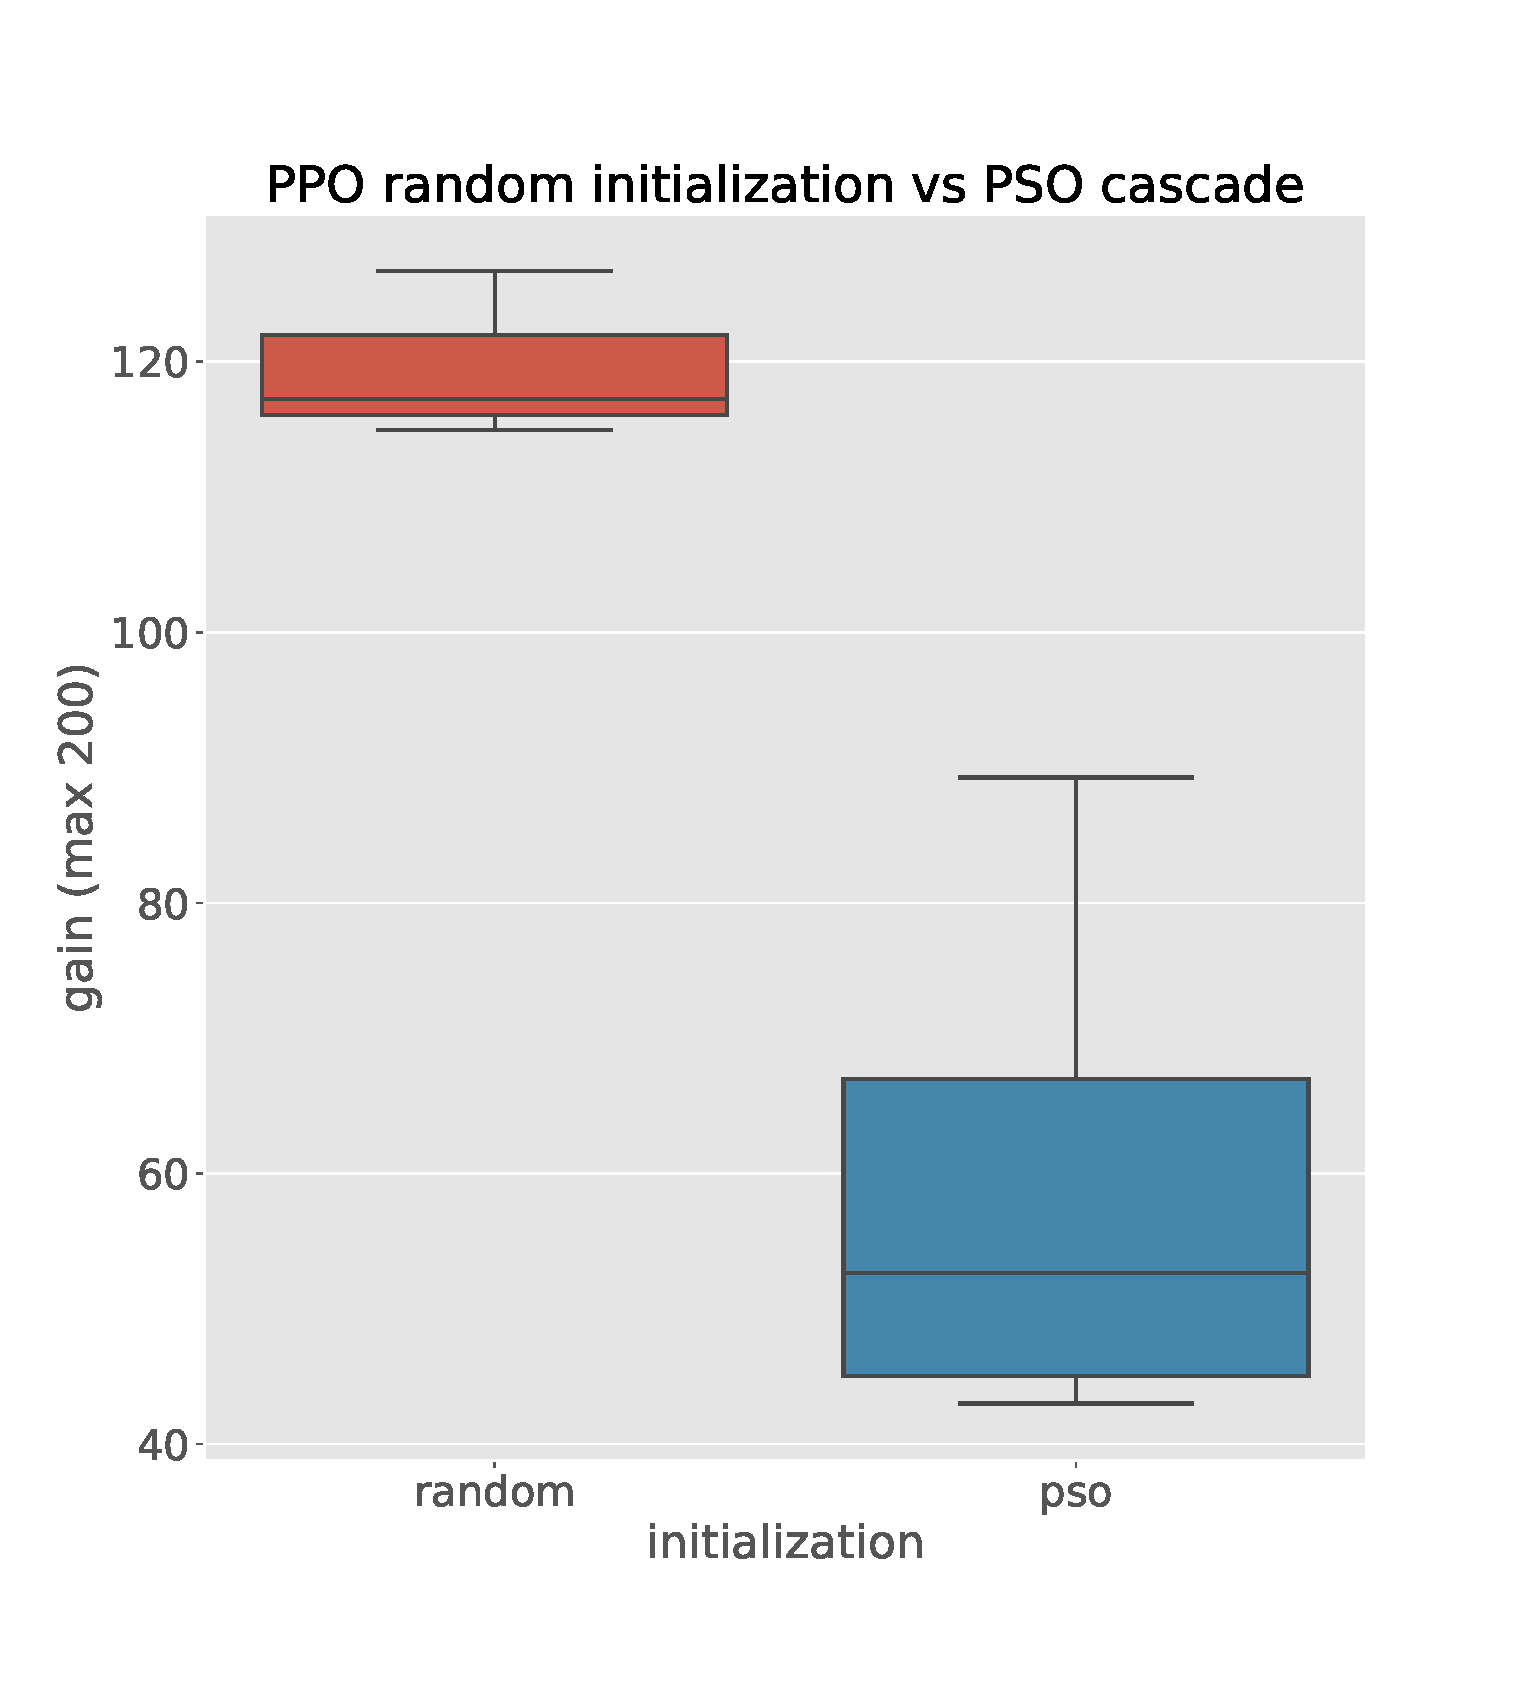
\includegraphics[width=0.5\textwidth]{images/random_vs_pso_initialization.eps}
        \caption{Gain comparison between PPO with random initialization and with PSO cascading.}
        \label{fig:random_vs_pso_initialization}
    \end{figure}
    Our explanation for getting worse results when using the technique mentioned above is that the function landscape is very big and PSO doesn't explore enough. Another possible explanation would be that the landscape is tricky when it comes to searching for generalist versus specialized solutions. We could try solving this problem by giving more exploratory power to PSO, but we did not experiment with this due to the lack of time.

    \subsection{PPO on the best configuration}\label{subsec:ppo-on-the-best-configuration}
    Considering the results above, we decided that PPO with random initialization and enemies \{1, 2, 6, 7\} chosen for training would be the best configuration. We ran 3000 epochs of this configuration, saving all the models along the way after every 250 epochs.
    After looking at the testing results, we noticed that the final gain is greater after 2000 epochs than after 3000 epochs (Fig.~\ref{fig:ppo_2000_vs_3000_epochs}).
    This means that there is overfitting during the training.
    We can conclude that by stopping the PPO algorithm after 2000 epochs instead of 3000 epochs
    we can end up with more generalized agents that perform better on average against all opponents.
    \begin{figure}[htbp]
        \centering
        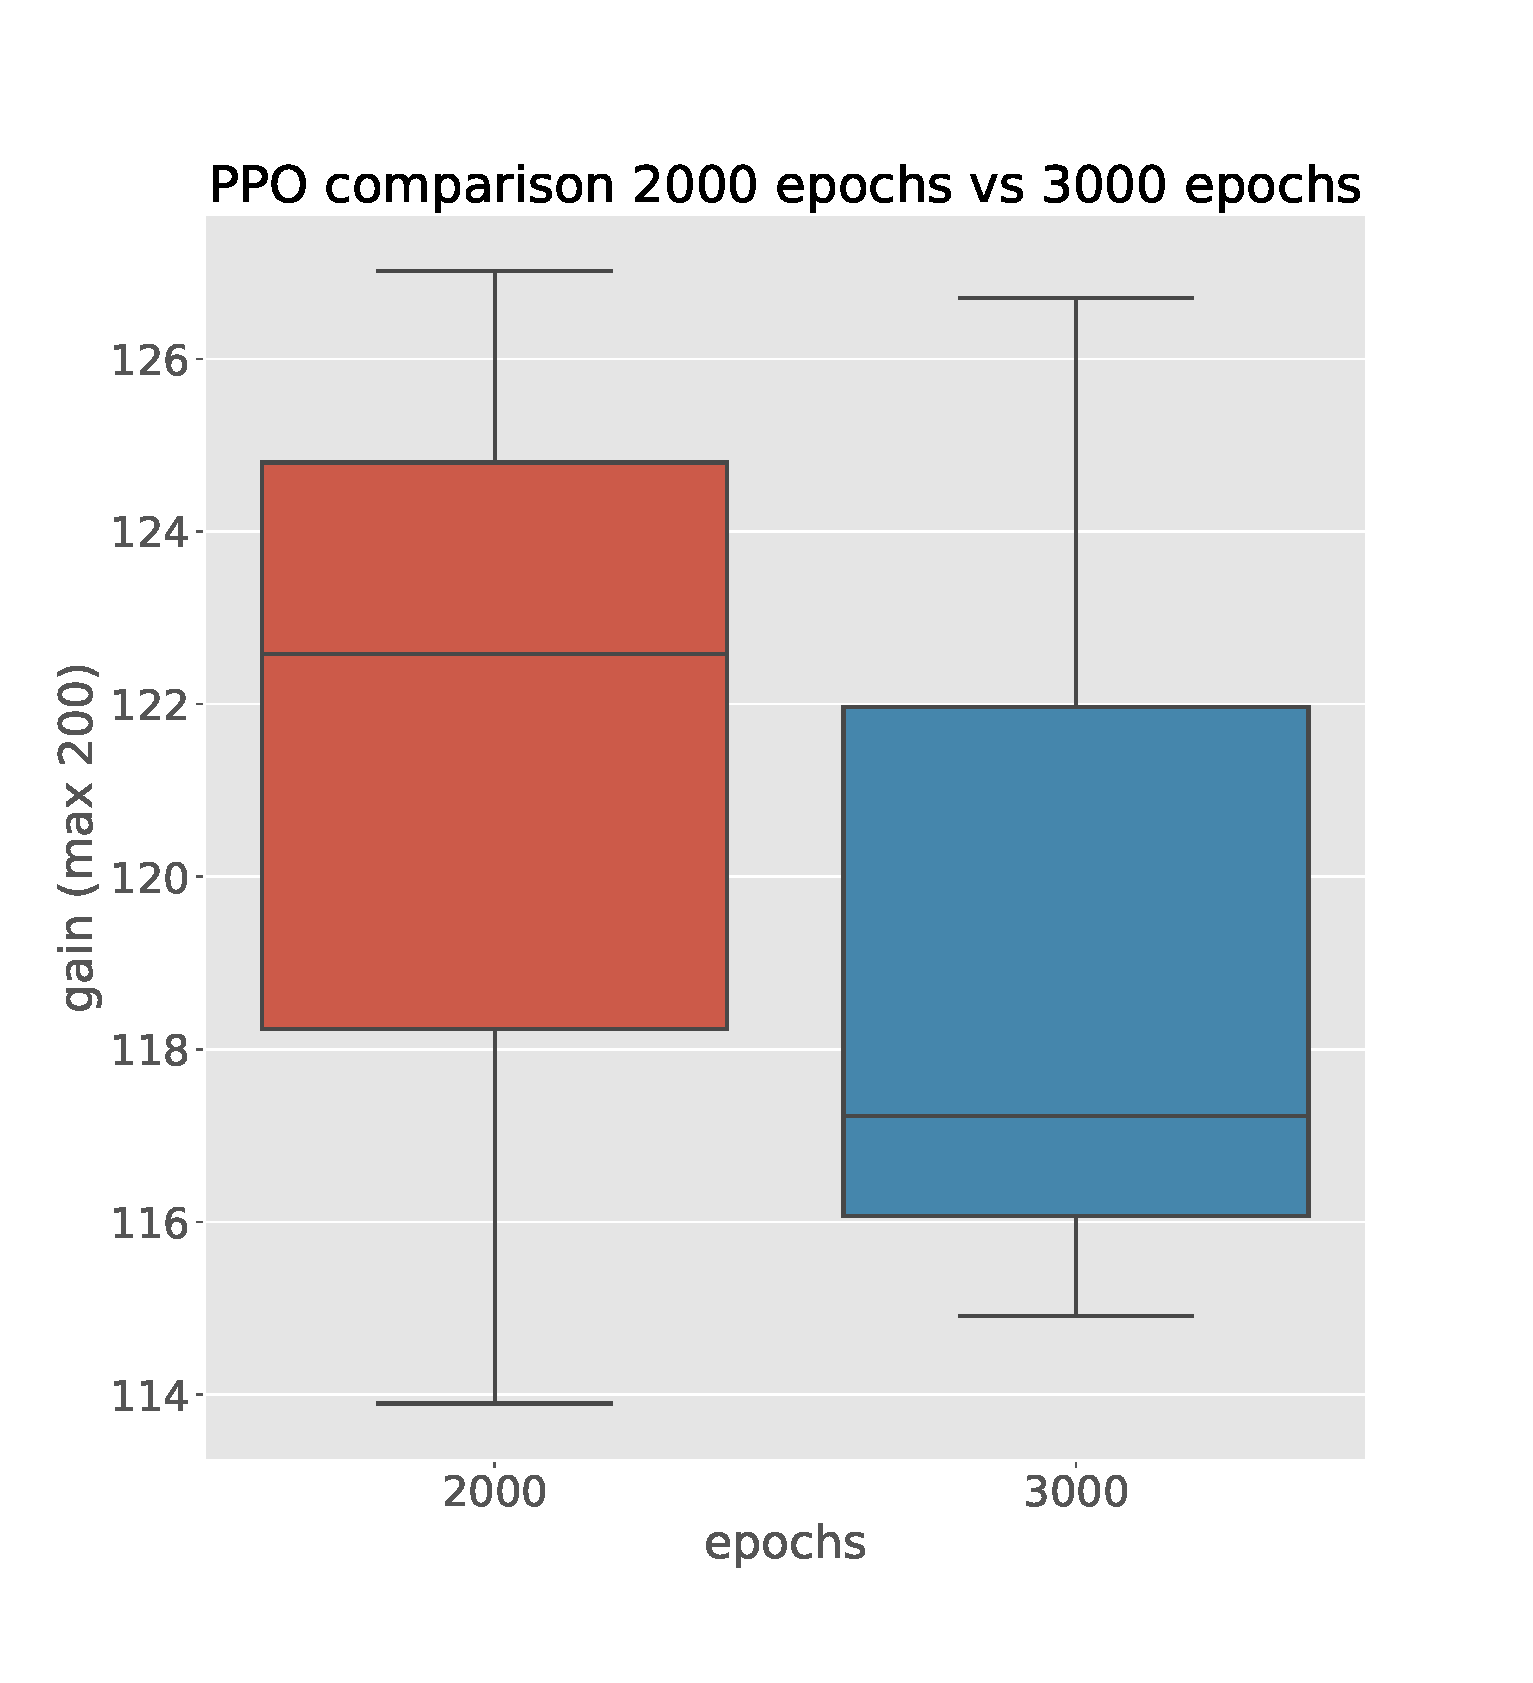
\includegraphics[width=0.5\textwidth]{images/ppo_2000_vs_3000_epochs.eps}
        \caption{Gain comparison between PPO after 2000 epochs and after 3000 epochs.}
        \label{fig:ppo_2000_vs_3000_epochs}
    \end{figure}

    \begin{figure}[htbp]
        \centering
        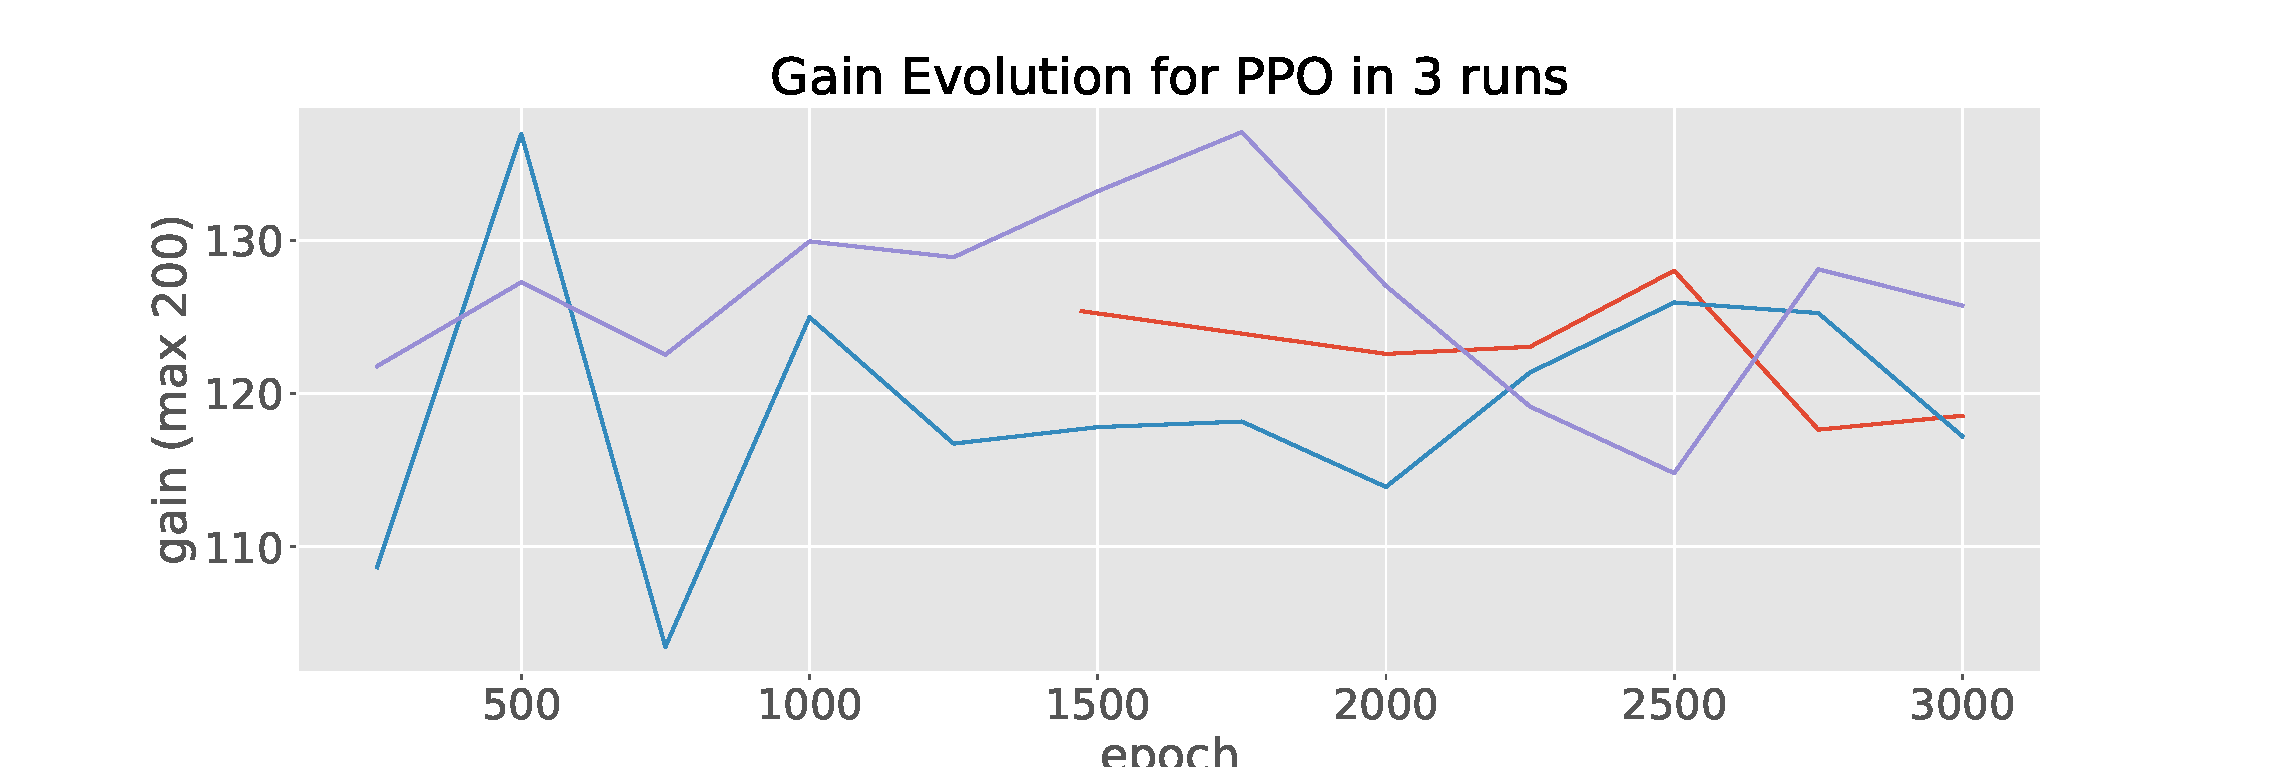
\includegraphics[width=0.5\textwidth]{images/ppo_gain_evolution_3_runs.eps}
        \caption{Gain Evolution for PPO in 3 runs, each model was ran 30 times on each opponent for calculating the gains}
        \label{fig:ppo_gain_evolution_3_runs}
    \end{figure}

    \subsection{Best Train Agent vs Best Tested Agent}\label{subsec:best-tested-agent}
    The best train gain was obtained in the first run of the PPO with random initialization.
    The train gain was computed as the harmonic mean of the averages per opponent of the 30 games played against
    the enemies \{1, 2, 6, 7\}.
    The highest train gain is 198.4.
    When computed against all opponents, this agent has an overall gain of 117.22.
    Out of the three PPO with random initialization runs, the highest final gain is 127.01.
    After the experiments were concluded we also looked at the overall gains of the agents before 3000 epochs (Fig.~\ref{fig:ppo_gain_evolution_3_runs}).
    For the runs 2 and 3 the snapshots of the models were saved every 250 epochs.
    In the first run these periodic snapshots start after 2000 epochs.
    When looking at the results of the intermediary agents we observed that there are some high peaks in test gain.
    The highest test gain was observed during the third run after 1750 epochs and it has a value of 137.18.


    \subsection{Comparison with the Upper Bound}\label{subsec:comparison-with-the-upper-bound}
    With the PPO algorithm trained on the opponents \{1, 2, 6, 7\} we have
    beat the best specialized models from the original paper which were given as upper bounds\cite{evoman}.


    \begin{table}[htbp]
        \caption{Specialized NEAT vs Generalized PPO (Gain)}
        \begin{center}
            \begin{tabular}{|c|c|c|c|c|c|}
                \hline
                \textbf{Opponent}&\multicolumn{4}{|c|}{\textbf{PPO}}&\textbf{Specialized} \\
                \cline{2-5}
                & \textbf{\textit{Run 1}}& \textbf{\textit{Run 2}}& \multicolumn{2}{|c|}{\textbf{\textit{Run 3}}} & NEAT \\
                \cline{4-5}
                & 3000 ep & 3000 ep & 3000 ep & 1750 ep & \\
                & (best at training) & & & (best tested) & \\
                \hline
                1 & 198.41 & 199.07 & 199.81 & 199.61 & 190.01 \\
                2 & 199.74 & 199.27 & 190.34 & 189.14 & 194.01 \\
                3 & 58.94 & 46.67 & 70.27 & 85.01 & 180.01 \\
                4 & 58.34 & 66.5 & 64.11 & 80.17 & 194.01 \\
                5 & 172.61 & 165.65 & 174.61 & 158.83 & 194.01\\
                6 & 195.73 & 196.95 & 195.85 & 194.37 & 173.01 \\
                7 & 199.79 & 195.05 & 193.27 & 191.17 & 177.01 \\
                8 & 122.17 & 145.49 & 141.89 & 140.61 & 186.01 \\
                \hline
                \textbf{\{1, 2, 6, 7\}} & & & & & \\
                \textbf{harmonic mean} & 198.4 & 197.57 & 194.75 & 193.49 & 183.09 \\
                \hline
                \textbf{final} & & & & & \\
                \textbf{harmonic mean} & 117.22 & 114.91 & 127.01 & 137.18 & 185.67\\
                \hline

            \end{tabular}
            \label{tab1}
        \end{center}
    \end{table}


    \begin{table}[htbp]
        \caption{Specialized NEAT vs Generalized PPO (Percentage of games won)}
        \begin{center}
            \begin{tabular}{|c|c|c|c|c|}
                \hline
                \textbf{Opponent}&\multicolumn{4}{|c|}{\textbf{PPO}} \\
                \cline{2-5}
                & \textbf{\textit{Run 1}}& \textbf{\textit{Run 2}}& \multicolumn{2}{|c|}{\textbf{\textit{Run 3}}} \\
                \cline{4-5}
                & 3000 ep & 3000 ep & 3000 ep & 1750 ep\\
                & (best at training) & & & (best tested) \\
                \hline
                1 & 100 & 100 & 100 & 100 \\
                2 & 100 & 100 & 100 & 100 \\
                3 & 3.33 & 0 & 3.33 & 46.66 \\
                4 & 0 & 6.66 & 0 & 6.66 \\
                5 & 100 & 96.66 & 100 & 100 \\
                6 & 100 & 100 & 100 & 100 \\
                7 & 100 & 93.33 & 100 & 100 \\
                8 & 80 & 100 & 96.66 & 90 \\
                \hline

            \end{tabular}
        \end{center}
    \end{table}

    \subsection{Time Analysis}\label{subsec:time-analysis}
    Since the match time is relevant, the machine on which the games were run is also relevant.
    The tests were run on an i7 4750HQ processor.
    The training was done on 3 threads.
    All computations were done on the CPU\@.
    The median game time during training is 28 seconds.
    The average number of frames per game is 287.

    \section{Conclusions}\label{sec:conclusions}
    After observing that the sparse methods were better than the iterative ones,
    PPO with random initialization is better than PSO cascaded with PPO and
    PPO with random initialization trained on four opponents leads to better train results
    than specialized agents trained with NEAT we can conclude that the problem space is in such a
    way that the methods with a greedy bias are moving away from the global optimum.

    \begin{thebibliography}{00}
        \bibitem{evoman_competition} Evoman: Game-playing Competition for WCCI 2020, \url{http://pesquisa.ufabc.edu.br/hal/Evoman.html}
        \bibitem{evoman} Fabricio Olivetti de Franca, Denis Fantinato, Karine Miras, A.E. Eiben and Patricia A. Vargas.
        "EvoMan: Game-playing Competition" arXiv:1912.10445
        \bibitem{karinemiras} de Araújo, Karine da Silva Miras, and Fabrício Olivetti de França.
        "An electronic-game framework for evaluating coevolutionary algorithms." arXiv:1604.00644 (2016).
        \bibitem{neuro} Floreano, D., Dürr, P. & Mattiussi, C. Neuroevolution: from architectures to learning. Evol. Intel. 1, 47–62 (2008). \url{https://doi.org/10.1007/s12065-007-0002-4}
        \bibitem{capcom} M. MEGA, "Produced by capcom, distributed by capcom, 1987," System: NES.
        \bibitem{q_learning} Watkins, C.J.C.H., Dayan, P. Q-learning. Machine Learning 8, 279–292 (1992)
        \bibitem{genetic_algorithm} Holland J.H., Genetic Algorithms and Adaptation. Adaptive Control of Ill-Defined Systems, 1984, Volume 16 ISBN 978-1-4684-8943-9
        \bibitem{pso} Kennedy, J.; Eberhart, R. (1995). "Particle Swarm Optimization". Proceedings of IEEE International Conference on Neural Networks. IV. pp. 1942–1948.
        \bibitem{neat} Kenneth O. Stanly; Rist Miikkulainen (2002). "Evolving Neural Networks through Augmenting Topologies". Evolutionary Computation, Volume 10, Issue 2, Summer 2002, p.99-127, \url{https://doi.org/10.1162/106365602320169811}
        \bibitem{ppo} John Schulman, Filip Wolski, Prafulla Dhariwal, Alex Radford, Oleg Klimov (2017) "Proximal Policy Optimization Algorithms", arXiv:1707.06347v2
        \bibitem{evoman_blog} Karine Miras, Evoman, \url{https://karinemirasblog.wordpress.com/portfolio/evoman/}
    \end{thebibliography}

\end{document}



